\vspace{0.015\textheight}
Possible biases in measurements, which can lead to significant deviations from the actual values, give rise to \newterm{systematic uncertainties}. Systematic uncertainties can arise from imperfections in the methodology, calibrations, and corrections. The following systematic uncertainties are studied and a scale for each uncertainty is derived using different techniques. Any correlation across bins is ignored and all errors are added in quadrature to calculate the total systematic uncertainty. We have followed standard practices of quoting systematic uncertainties. All systematic uncertainties quoted are one standard deviation ($\pm1\sigma$) unless described otherwise.

\section{Jet Energy Scale (JES)}
The uncertainty in determining corrections to jet energies (see Section \ref{sec:jet_identification}) is taken into account as it changes the signal acceptance and the trigger efficiency, and hence the measured kinematic distributions. Figure~\ref{fig:JESFracSyst} illustrates the fractional uncertainties associated with the jet energy corrections.

\begin{figure}[htb!m]
 \centering
 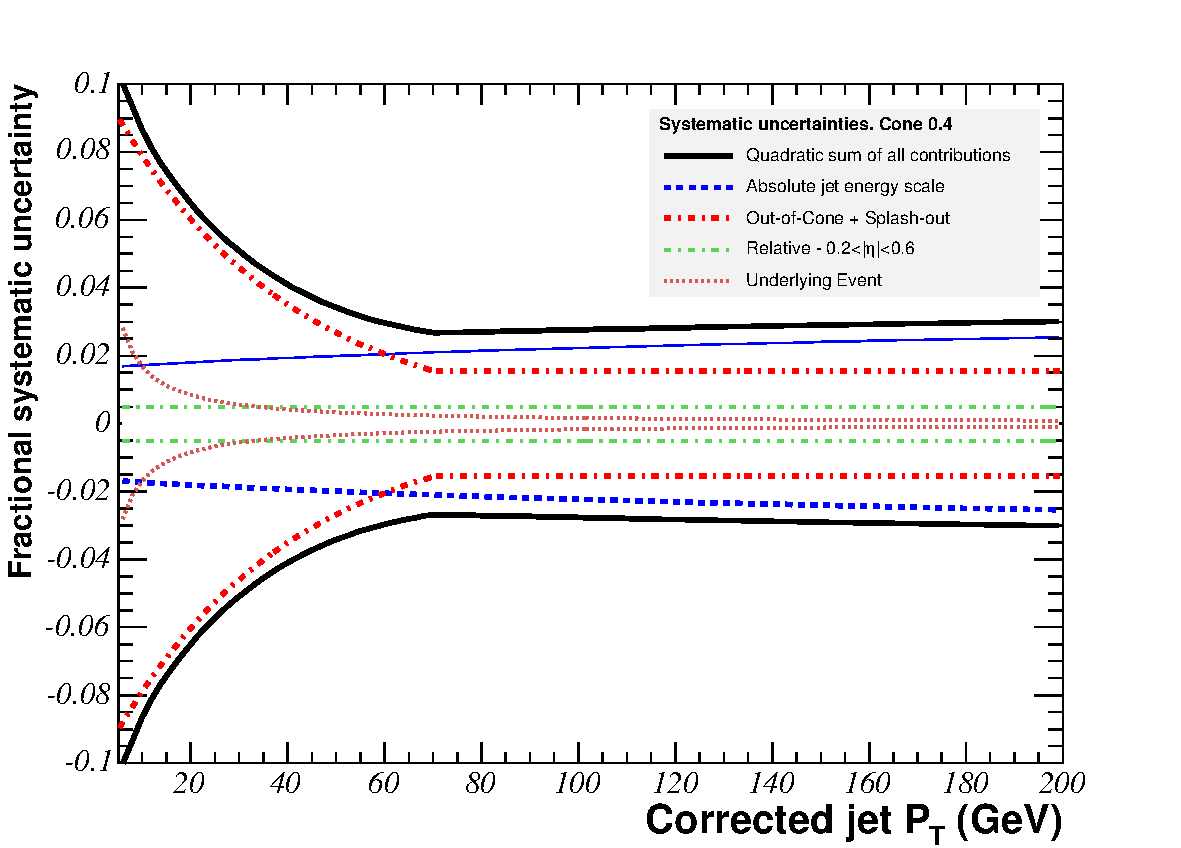
\includegraphics[scale=0.8]{./JES_FractioanlSystUncertainty.pdf}
 % JES_FractioanlSystUncertainty.pdf: 567x407 pixel, 72dpi, 20.00x14.36 cm, bb=0 0 567 407
 \caption{Scales of the uncertainties of individual jet energy corrections in the central calorimeter. The total uncertainty is obtained by adding individual corrections in quadrature.}
 \label{fig:JESFracSyst}
\end{figure}

Uncertainties due to jet energy mismeasurements are obtained by varying the corrected jet energy by one standard deviation from the mean corrected value, \mbox{+$\sigma$} and \mbox{--$\sigma$}. A new set of events are selected from this shifted jet energy data. Each variation is compared to the nominal value, and the  maximum deviation from the nominal value is taken as the systematic uncertainty. The jet energy scale is by far the largest uncertainty in most of the measured distributions.
%{\sc [TODO: image of photon Et spectrum central/jes up/jes down goes here]}

\section{Fake Photon Fraction}
The uncertainty in the determination of the true photon fraction is described in Appendix~\ref{app:CESCPRMtd} and is taken into account as follows.

The normalization of the QCD template and the SM prompt photon template is changed by $\pm\sigma = \pm 0.068$ from the nominal value of the fake photon fraction, which is defined in Eq.~\ref{eqa:FakeFraction}. For each histogram bin, the maximum difference between the nominal distribution and the two varied ($\pm \sigma$) distributions is taken as the systematic uncertainty. This uncertainty makes a moderate contribution to the total systematic uncertainty. This uncertainty increases from about 10\% to about 40\% with increasing photon \et.
%{\sc [TODO: image of photon Et spectrum central/fake fraction+sigma down goes here]}

\section{Choice of QCD Selection}
The uncertainty in the choice of photon sideband to represent the fake jets in the tight photon sample is estimated by varying the loose photon selection requirements to match the tight photon ID selection requirements. By doing so, one probes the sideband sample for the correlation to the tight photon sample. The selection requirements, Isolation Energy ($E_{T}^{\mathrm{Iso}}$), Had/Em ($E_{HAD}/E_{EM}$), Track \pt, and Track Isolation are common to both loose and tight photon selection requirements. Each of these loose photon selection requirements is set equal to the tight photon selection requirements one at a time, and four new sideband samples are selected. New samples are normalized back to the original (nominal) sideband sample and compared. The maximum deviation of each varied sample from the original sample is taken as the systematic uncertainty.
%[IMAGE FROM THE FINAL HIST ROOT FILE SHOWING THE QCD ID SYSTEMATIC SHOULD GO IN HERE]

\section{PDF Uncertainty}
The parton distribution in the proton and antiproton is described by the PDFs. (A PDF is a probability density function for finding a parton with a certain longitudinal momentum fraction $x$ at momentum transfer $Q^{2}$; see Section \ref{sec:pQCD}). Each PDF is defined by 20 eigenvectors that are derived from measurements obtained from various previous experiments. The acceptance and trigger efficiency depends on the PDFs. The uncertainty in the PDFs used in MC event generation is derived following the recommendations of the CDF Joint Physics Group \cite{www:JPforPDFsyst, cdfnote:7051}.

Instead of generating many different sets of \MC event samples for each PDF set, {\sc CTEQ5L} events are reweighted to {\sc CTEQ6M} (next-to-leading order PDFs). The initial parton's information is approximated using generator-level information and 40~(+1) weights are generated for each of the 20 eigenvectors (higher and lower than nominal) and for a base distribution. Each kinematic distribution is remade according to the 40~(+1) generated weights. A maximum of 2 variations for each weight (representing an eigenvector) are added in quadrature to derive the total uncertainty. They are added in quadrature because these 20 eigenvectors are independent. A set of sample distributions in Fig.~\ref{fig:PDFsyst} illustrates the size of this uncertainty.

%This assumes when generating many different \MC event samples to estimate the PDF uncertainty would be due to the difference in the PDFs.
\begin{figure}[p]
 \centering
 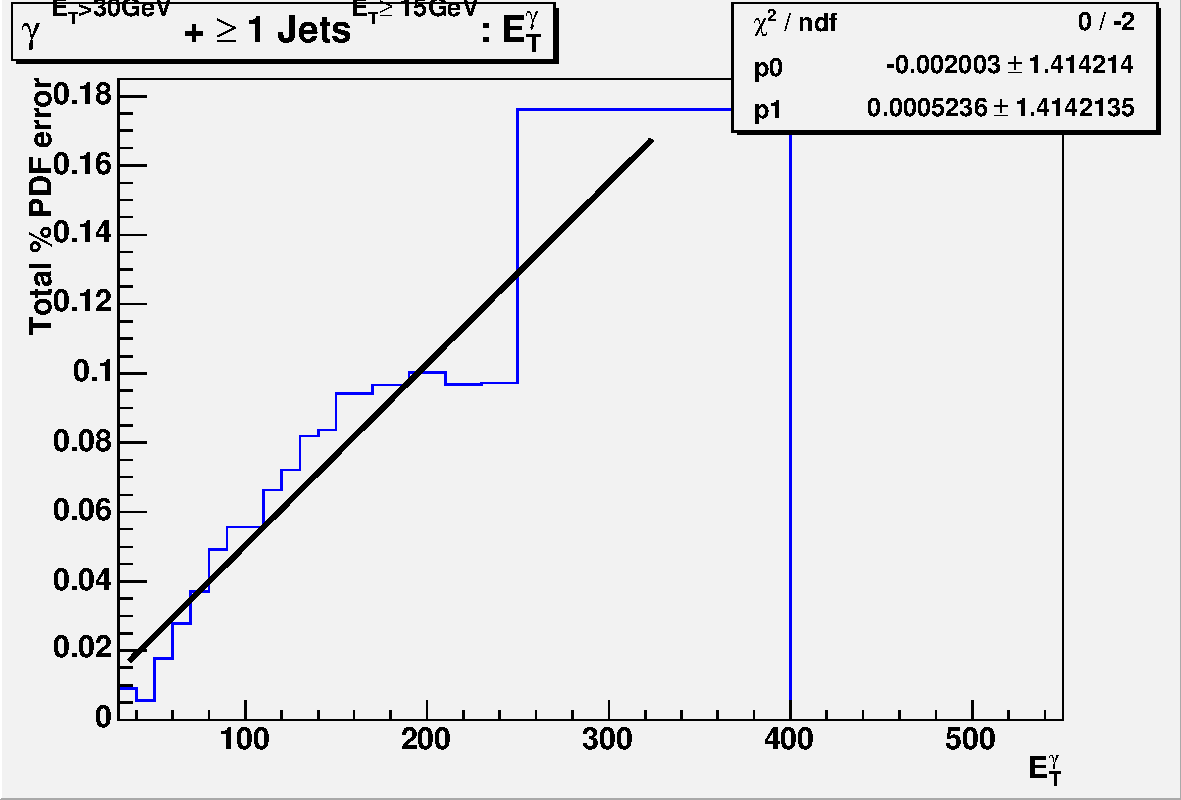
\includegraphics[scale=0.36,keepaspectratio=true]{PDFsyst_pj1_Et_pho.pdf}\hspace{2ex}
 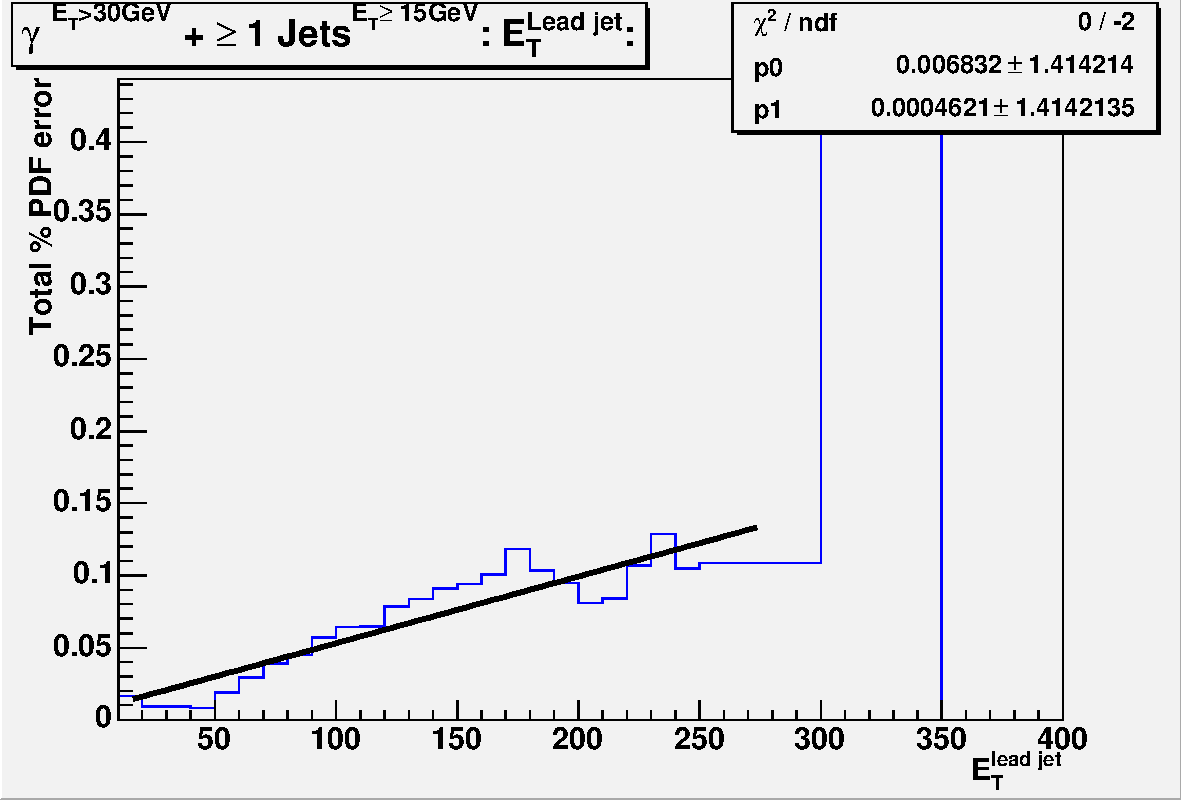
\includegraphics[scale=0.36,keepaspectratio=true]{PDFsyst_pj1_Et_leadjet.pdf}
\\[2ex]
 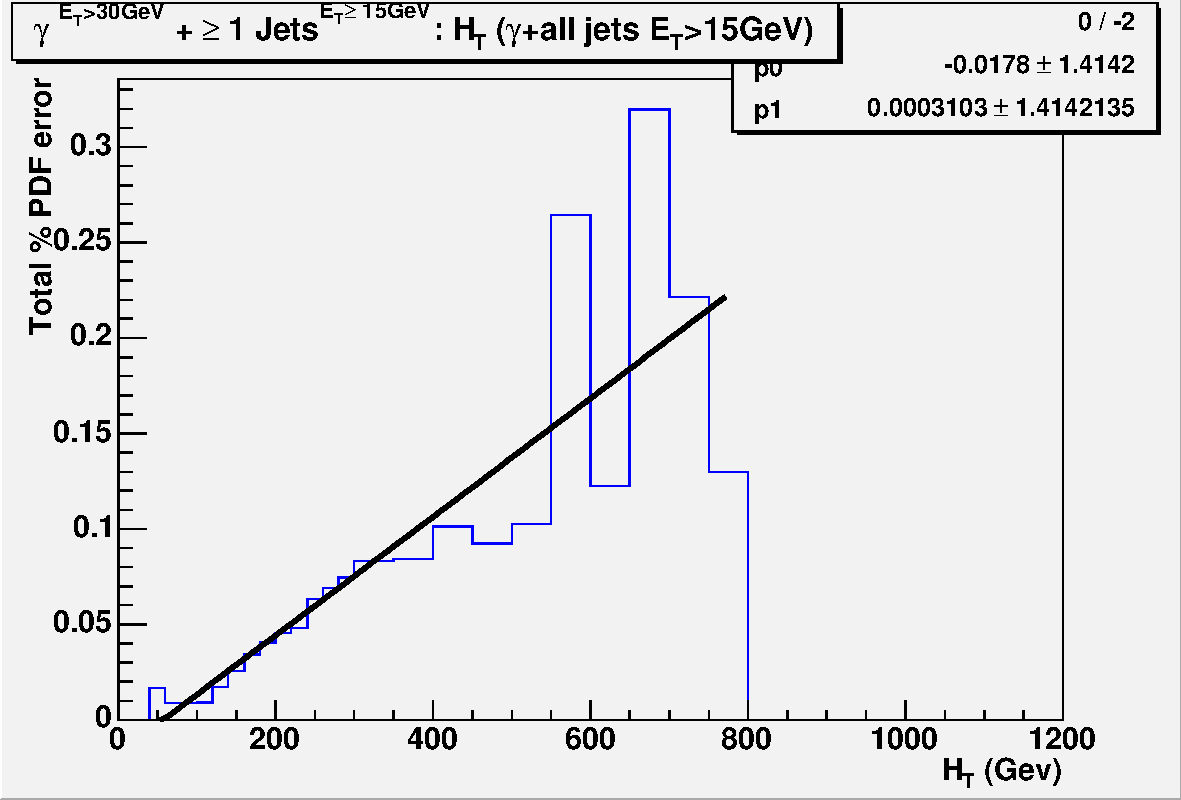
\includegraphics[scale=0.36,keepaspectratio=true]{PDFsyst_pj1_Ht.pdf}\hspace{2ex}
 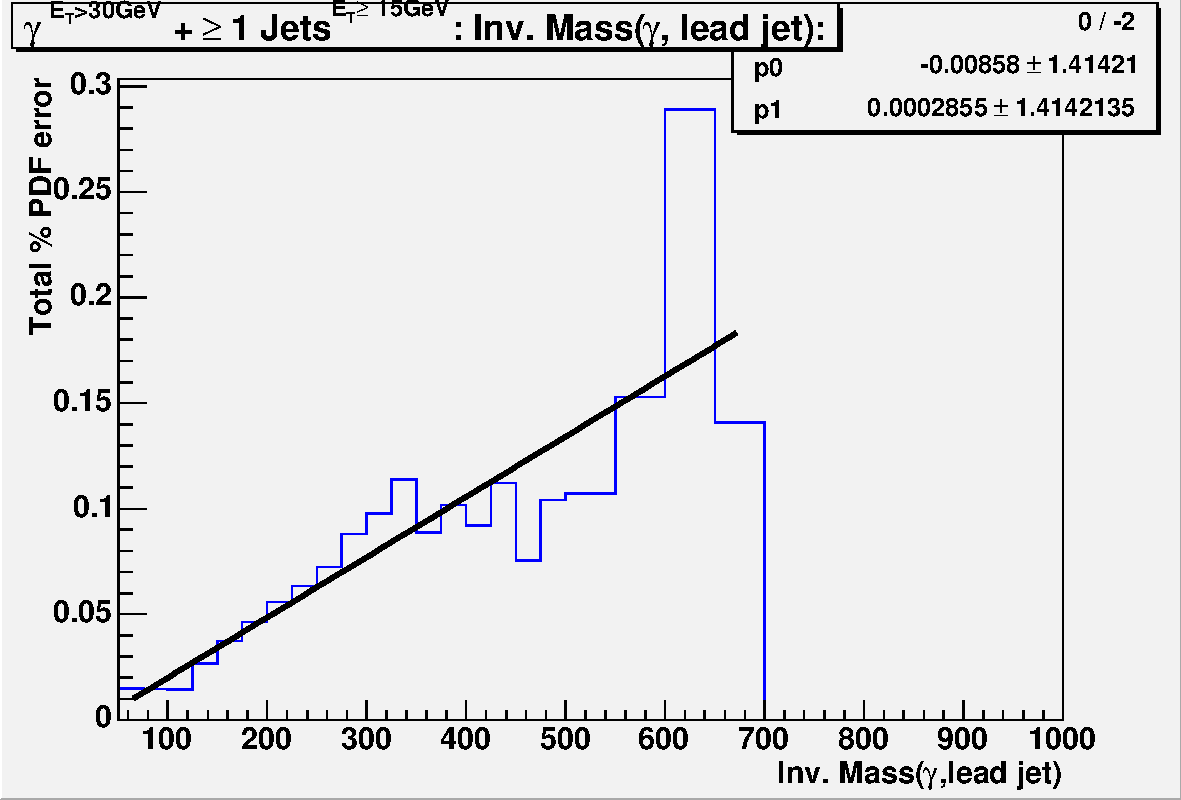
\includegraphics[scale=0.36,keepaspectratio=true]{PDFsyst_pj1_InvM_phojet.pdf}
 \caption{Scale of the total percentage PDF uncertainty for different kinematic distributions in the \phoonejet event sample. The distributions are fitted with a first-order polynomial and used to derive the uncertainty in the final (result) distributions. The function is evaluated at the bin center when deriving the uncertainty for a bin. The total uncertainty ranges from a few percent to about 20\%. The minimum uncertainty is set to be 1\%.}
 \label{fig:PDFsyst}
\end{figure}

\section{Renormalization, Factorization, and Fragmentation Scale Dependence}
The dependence on the renormalization, factorization, and fragmentation scales (Q$^{2}$) are varied to estimate the higher-order contributions not considered by using leading-order MC signal sample. Two MC samples are generated by varying the nominal scale by 0.5 and 2.0. Each varied sample is normalized back to the nominal sample and the difference in shape from the nominal shape is taken as the systematic uncertainty. This systematic uncertainty is derived using only the generator-level objects. The leading photon is identified using generator-level information and hadron-level jets are used. A set of sample distributions in Fig.~\ref{fig:Q2Syst} illustrates the scale of this uncertainty.

\begin{figure}[p]
 \centering
 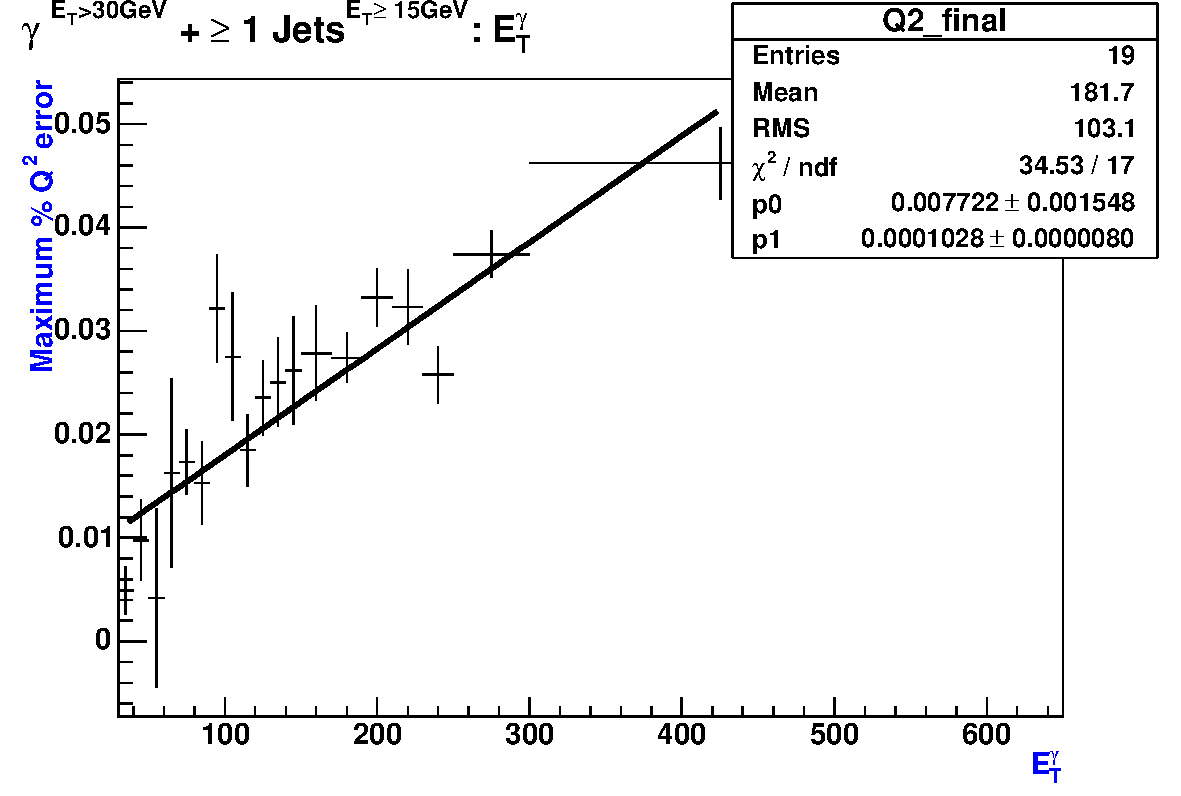
\includegraphics[scale=0.36,keepaspectratio=true]{Q2syst_pj1_Et_pho.pdf}\hspace{2ex}
 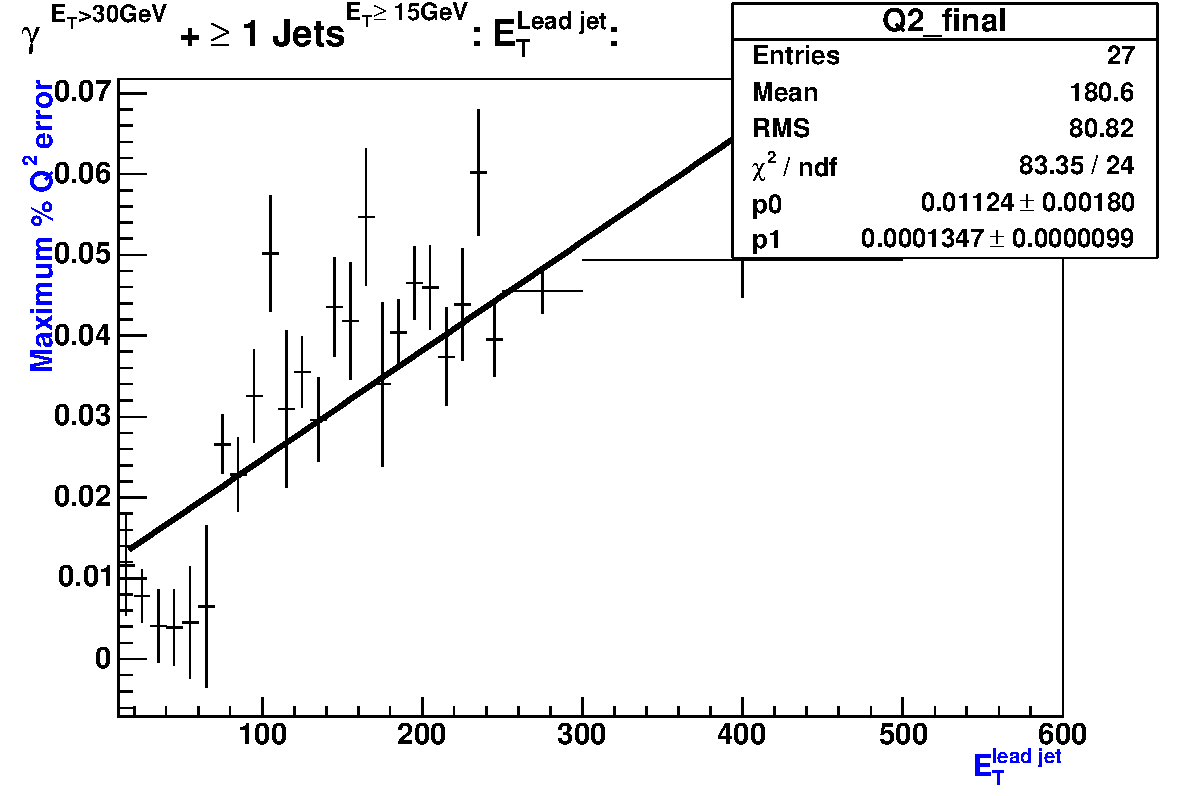
\includegraphics[scale=0.36,keepaspectratio=true]{Q2syst_pj1_Et_leadjet.pdf}\\[2ex]
 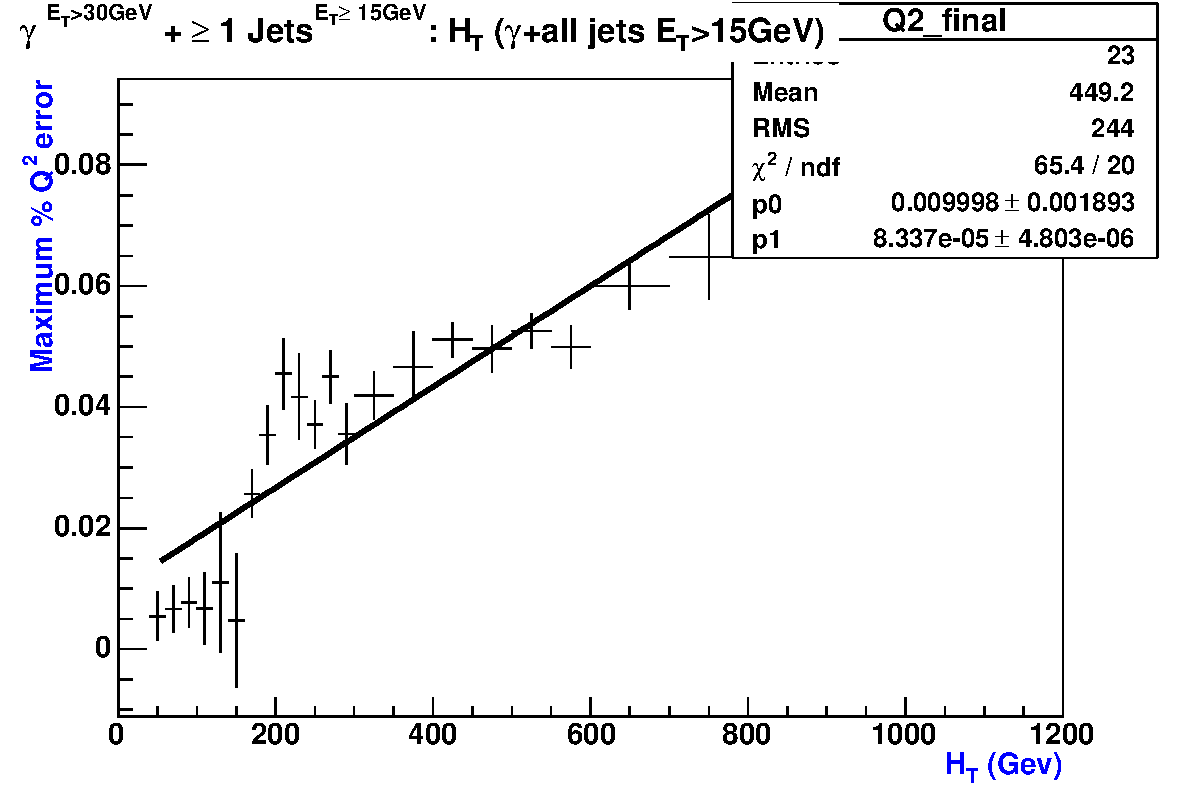
\includegraphics[scale=0.36,keepaspectratio=true]{Q2syst_pj1_Ht.pdf}\hspace{2ex}
 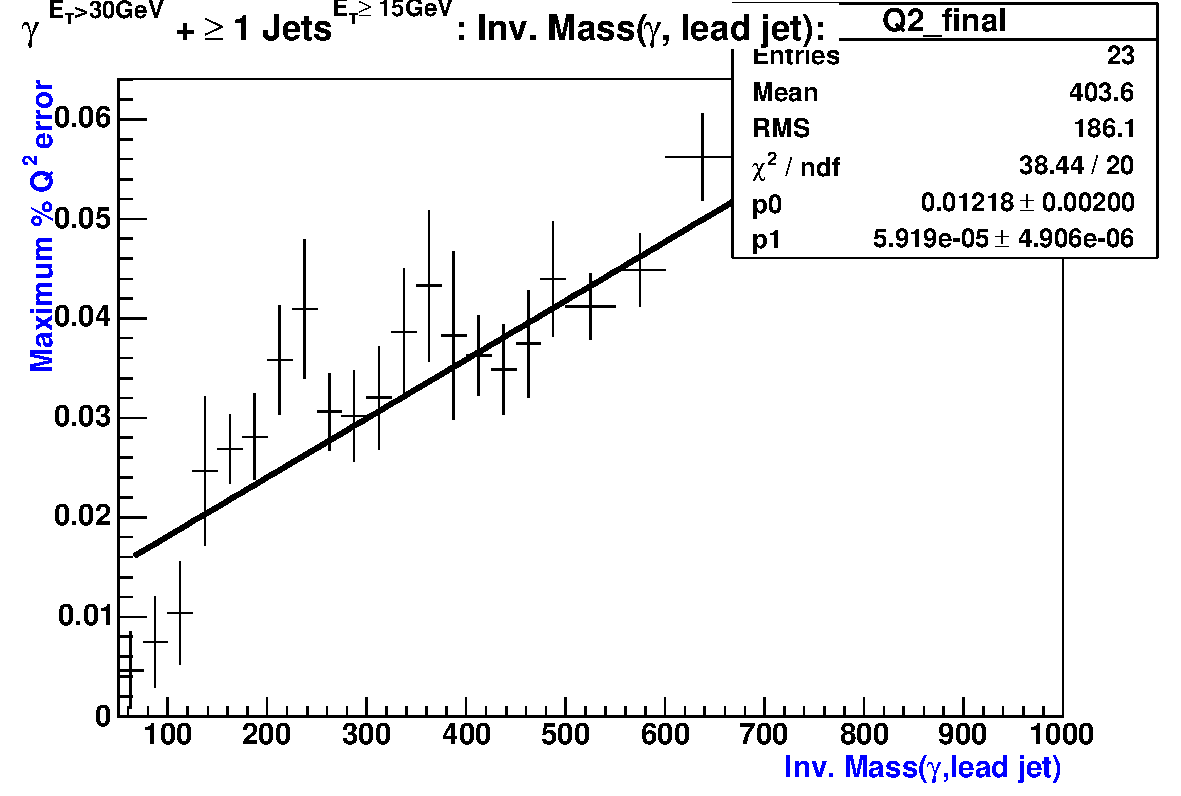
\includegraphics[scale=0.36,keepaspectratio=true]{Q2syst_pj1_InvM_phojet.pdf}
 \caption{Scale of the total percentage $Q^{2}$ uncertainty for different kinematic distributions in the \phoonejet event sample. The distributions are fitted with a first-order polynomial and used to derive the uncertainty in the final (result) distributions. The function is evaluated at the bin center when deriving the uncertainty for a bin. The total uncertainty ranges from a few percent to about 10\%. The minimum uncertainty is set to be 1\%.}
 \label{fig:Q2Syst}
\end{figure}

\section{Initial State Radiation (ISR) and Final State Radiation (FSR) Effects}
%this changes the Sudakov form factors. should I use that word? then need to explain the origin etc.
Uncertainty in the the amount of radiation from the incoming and outgoing partons is estimated by varying the corresponding \pythiaText parameters following the Joint Physics Group's recommendations \cite{www:JPforISRFSRsyst}. Five MC samples (more ISR, less ISR, more FSR, less FSR, and nominal) were needed. Table~\ref{tab:pythiaISRFSRParamList} describes the \pythiaText parameters modified in order to generate those event samples. The MC samples for each variation are really a combination of many different MC sample with different $\hat{p}_{T}$, which are normalized by cross section to get the complete spectrum. Each of the four variations is normalized to the nominal distribution and the maximum variation of ISR and FSR is added in quadrature to derive the total systematic uncertainty.

\begin{table}[p]
\caption{\pythiaText parameters used with PARP(3)=1 to generate different MC samples to derive the ISR/FSR systematic uncertainties.}
\label{tab:pythiaISRFSRParamList}
\centering
\begin{tabular}{cc}
\hline
\BUbf{MC Sample} & \BUbf{\pythiaText Parameters and Values}\\
\hline
nominal (default) ISR sample 	& PARP(61)=0.146, PARP(64)=1.0\\
more ISR sample 		& PARP(61)=0.292, PARP(64)=0.5\\
less ISR sample 		& PARP(61)=0.073, PARP(64)=2.0\\
nominal (default) FSR sample 	& PARP(72)=0.146, PARP(71)=4.0\\
more FSR sample 		& PARP(72)=0.292, PARP(71)=8.0\\
less FSR sample 		& PARP(72)=0.073, PARP(71)=2.0\\
\hline
\end{tabular}
\end{table}
%A set of sample distributions in Fig.~\ref{fig:ISRFSRSyst} illustrates the scale of this uncertainty.
%[THE IMAGES DOES NOT LOOK PRETTY. SHOULD I INCLUDE THEM? IF NOT SHOULD I TAKE OUT ALL THE IMAGES SHOWN UNDER OTHER SYSTEMATIC ERRORS?]
% \begin{figure}[h!]
% \centering
% 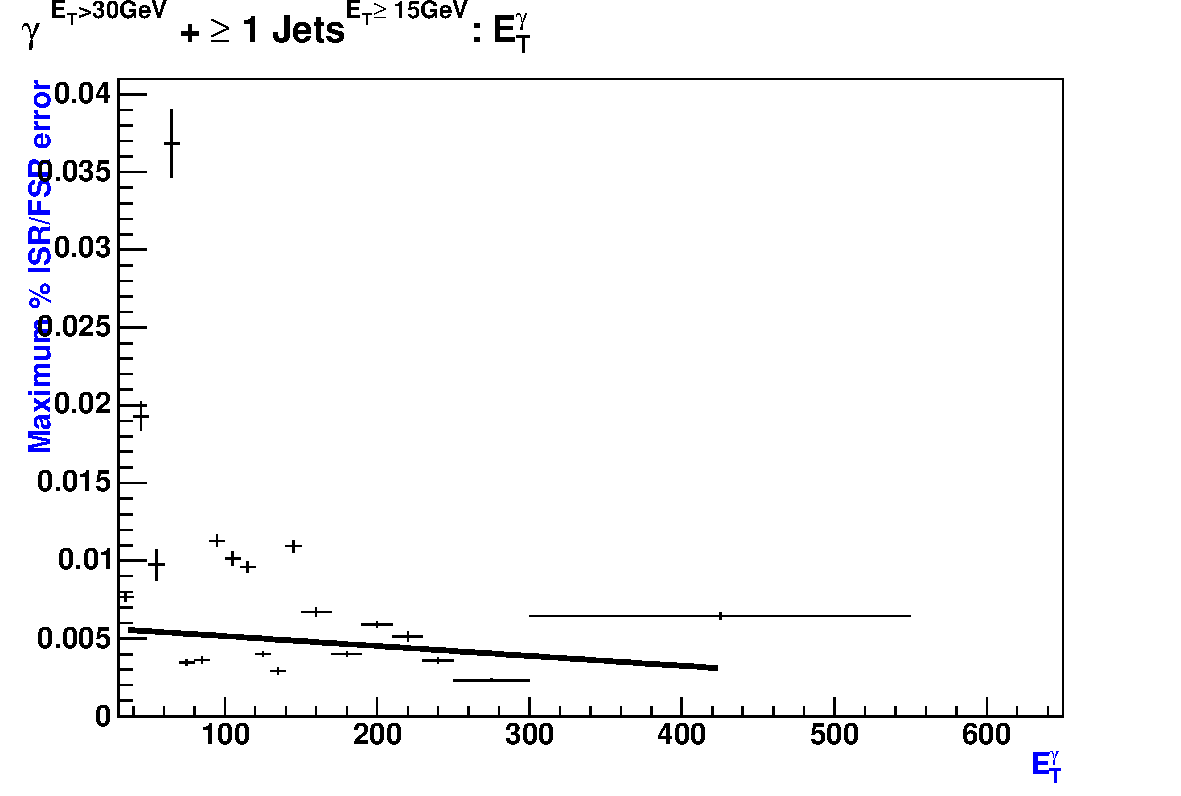
\includegraphics[scale=0.25,keepaspectratio=true]{IsrFsrSyst_pj1_Et_pho.pdf}
% 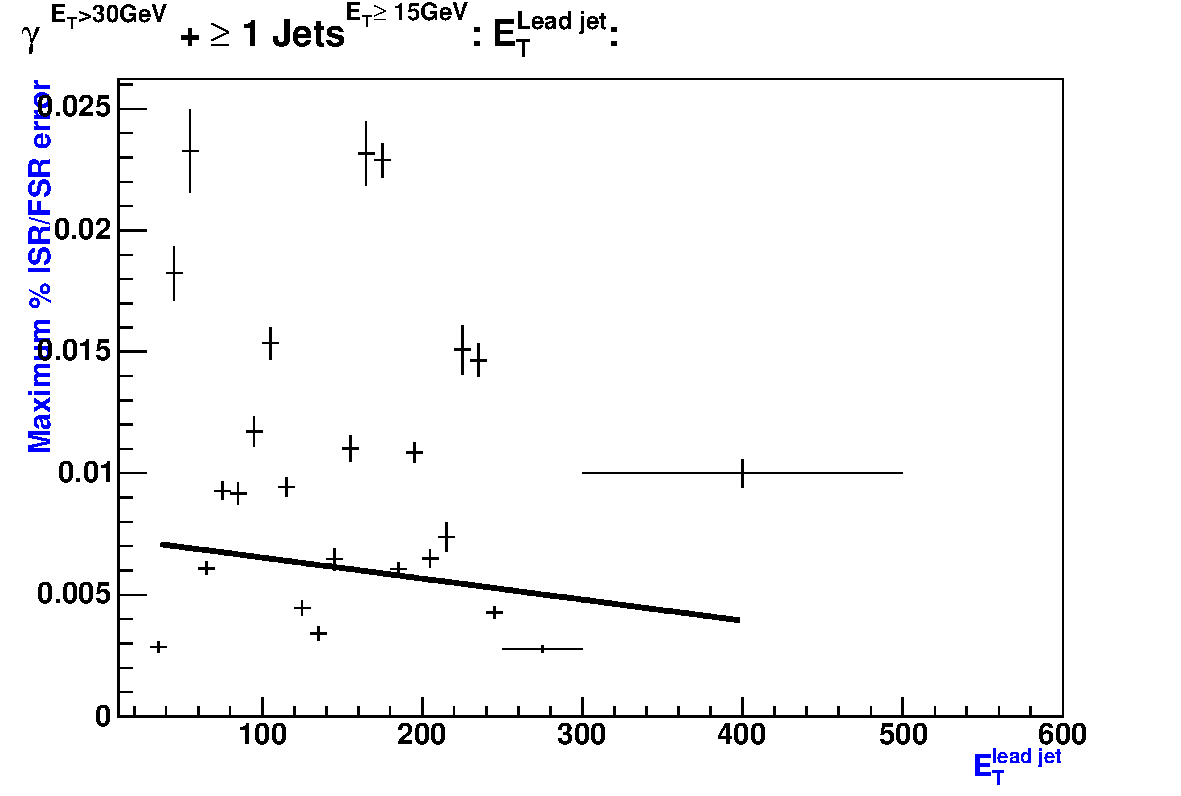
\includegraphics[scale=0.25,keepaspectratio=true]{IsrFsrSyst_pj1_Et_leadjet.pdf}
% 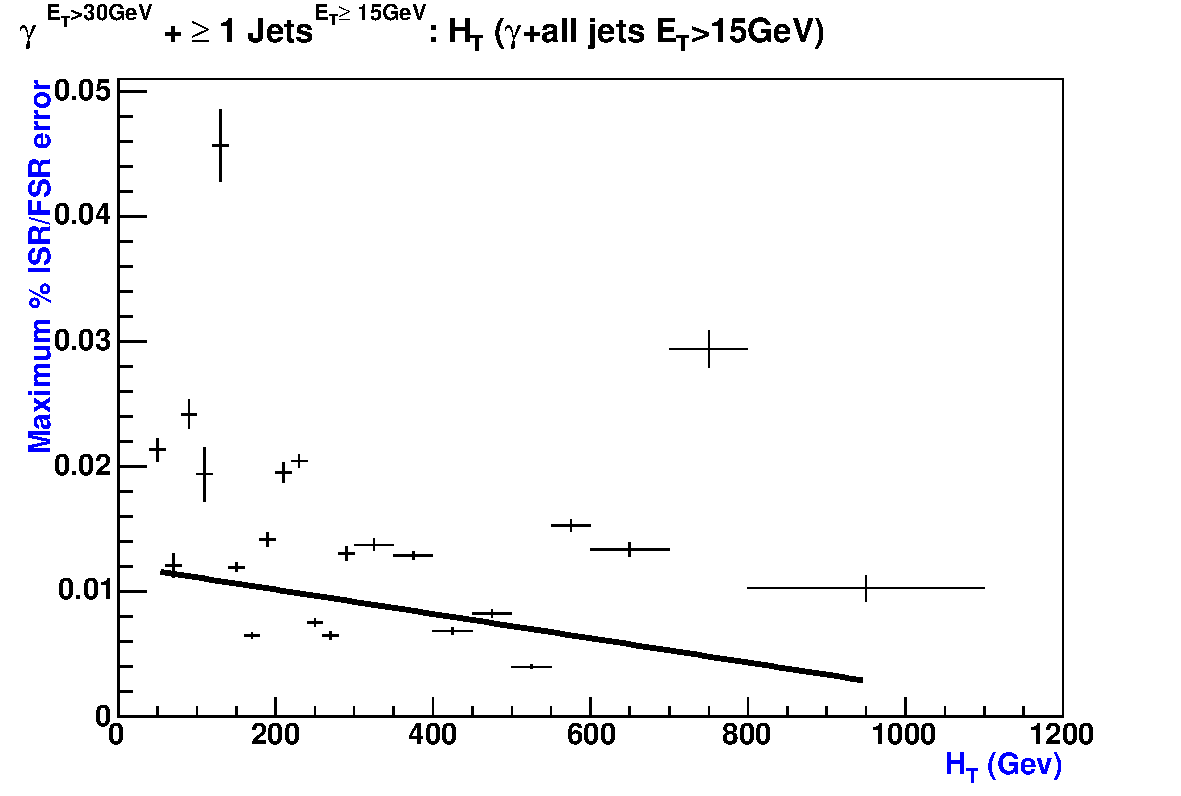
\includegraphics[scale=0.25,keepaspectratio=true]{IsrFsrSyst_pj1_Ht.pdf}
% 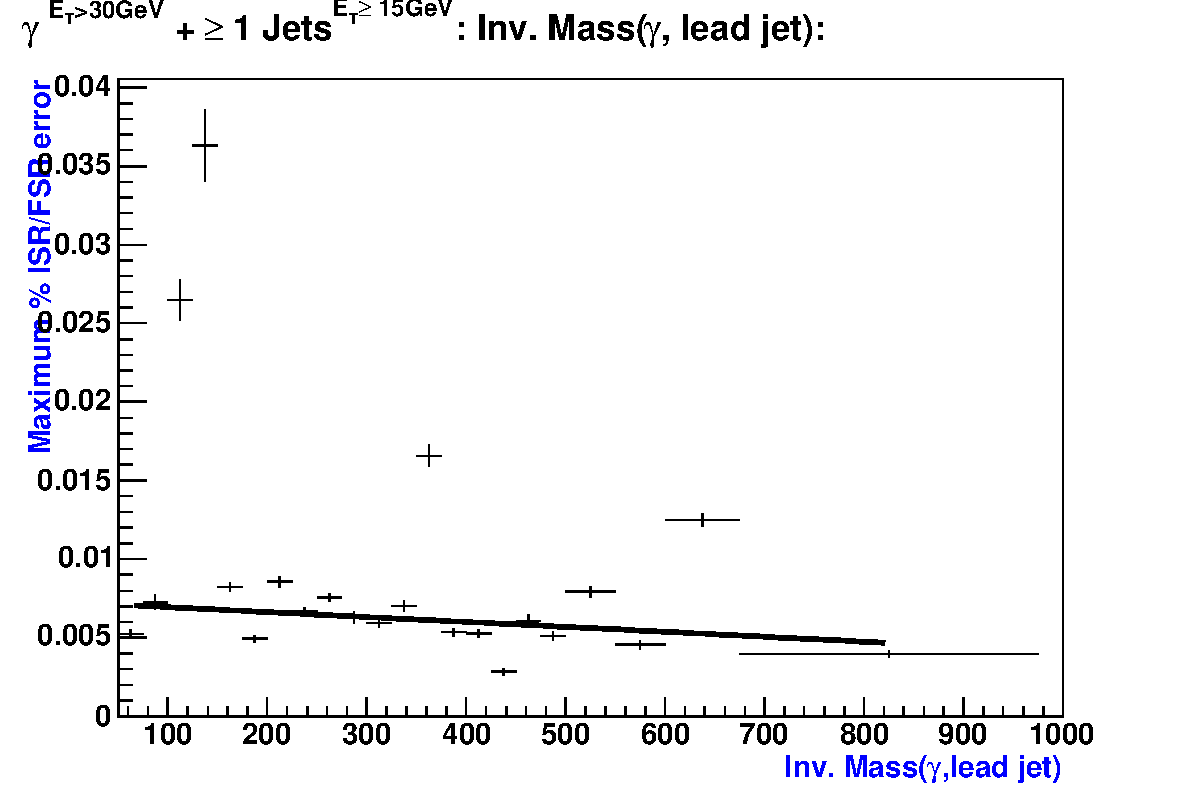
\includegraphics[scale=0.25,keepaspectratio=true]{IsrFsrSyst_pj1_InvM_phojet.pdf}
% \caption{Scale of the total percentage ISR/FSR uncertainty for different kinematic distributions in \phoonejet event sample. A first order polynomial is fitted and used to derive the uncertainty in the final (results) distributions. The function is evaluated at the bin center when deriving uncertainty for a bin. The total uncertainty ranges from few percent to about 10\%. The minimum uncertainty is set to be 1\%.}
% \label{fig:ISRFSRSyst}
% \end{figure}

\section{Uncertainty in the Strong Coupling Constant ($\alpha_s$)}
The value of the strong coupling constant used in the generation of \MC event samples is not measured directly or absolutely. It is measured at the masses of the \pizero and $Z$-boson and then extrapolated to the other regions. An uncertainty for this is derived by comparing CTEQ5L PDF-based \MC events to MRST98 PDF-based \MC events, which use different values of \alphas when generating events. A set of sample distributions in Fig.~\ref{fig:AlphaS_Syst} illustrates the size of this uncertainty.

\begin{figure}[h!]
 \centering
 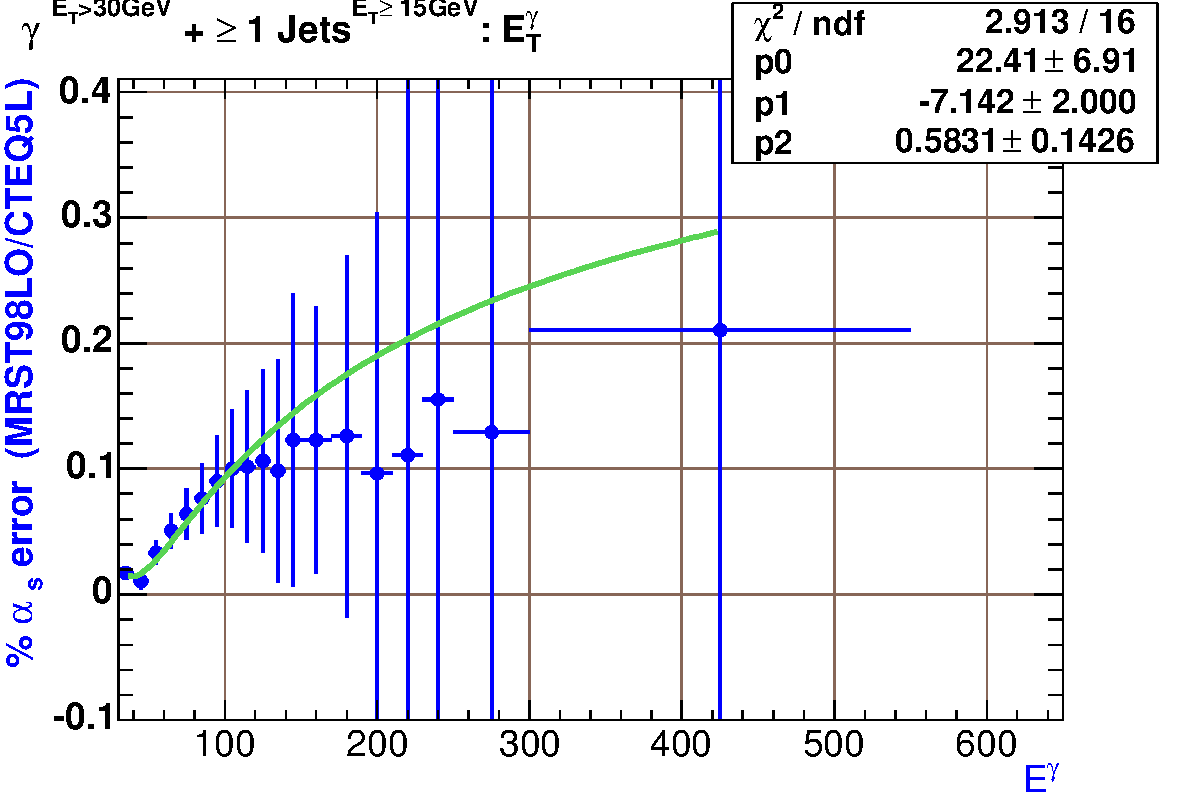
\includegraphics[scale=0.36,keepaspectratio=true]{AlphaSsyst_pj1_Et_pho.pdf}\hspace{2ex}
 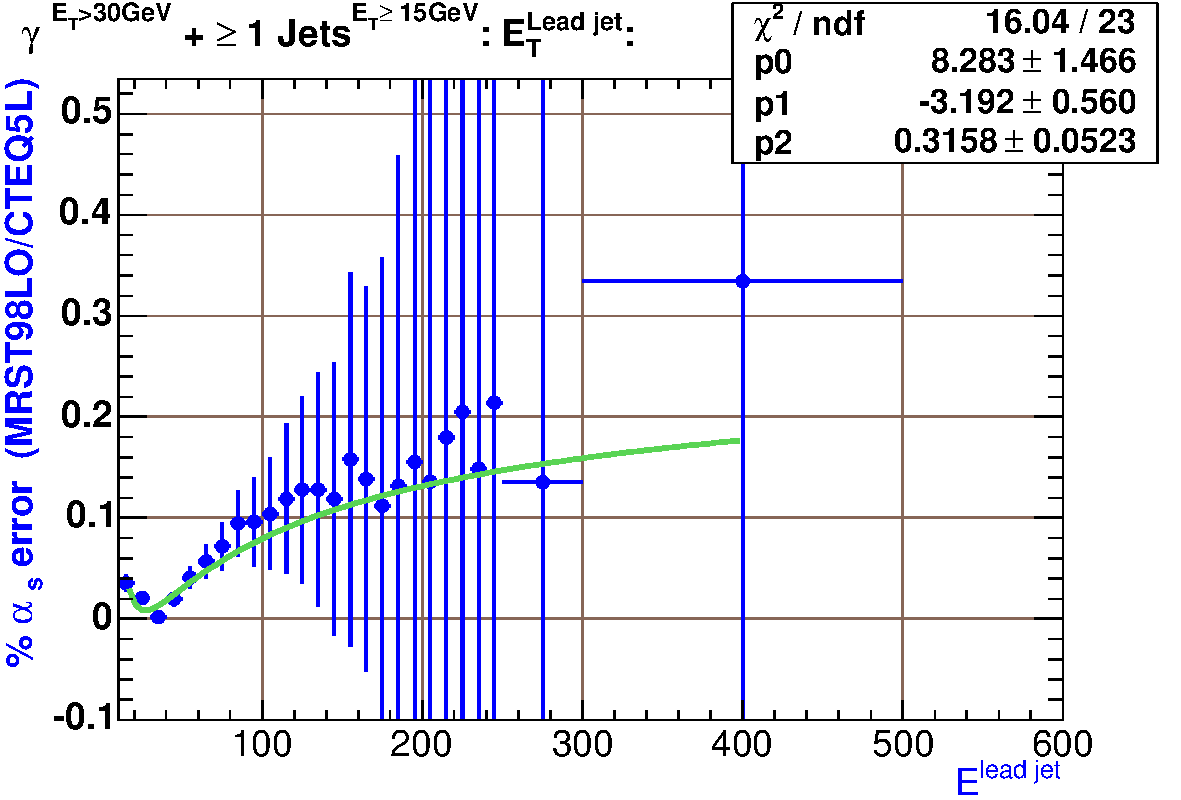
\includegraphics[scale=0.36,keepaspectratio=true]{AlphaSsyst_pj1_Et_leadjet.pdf}\\[2ex]
 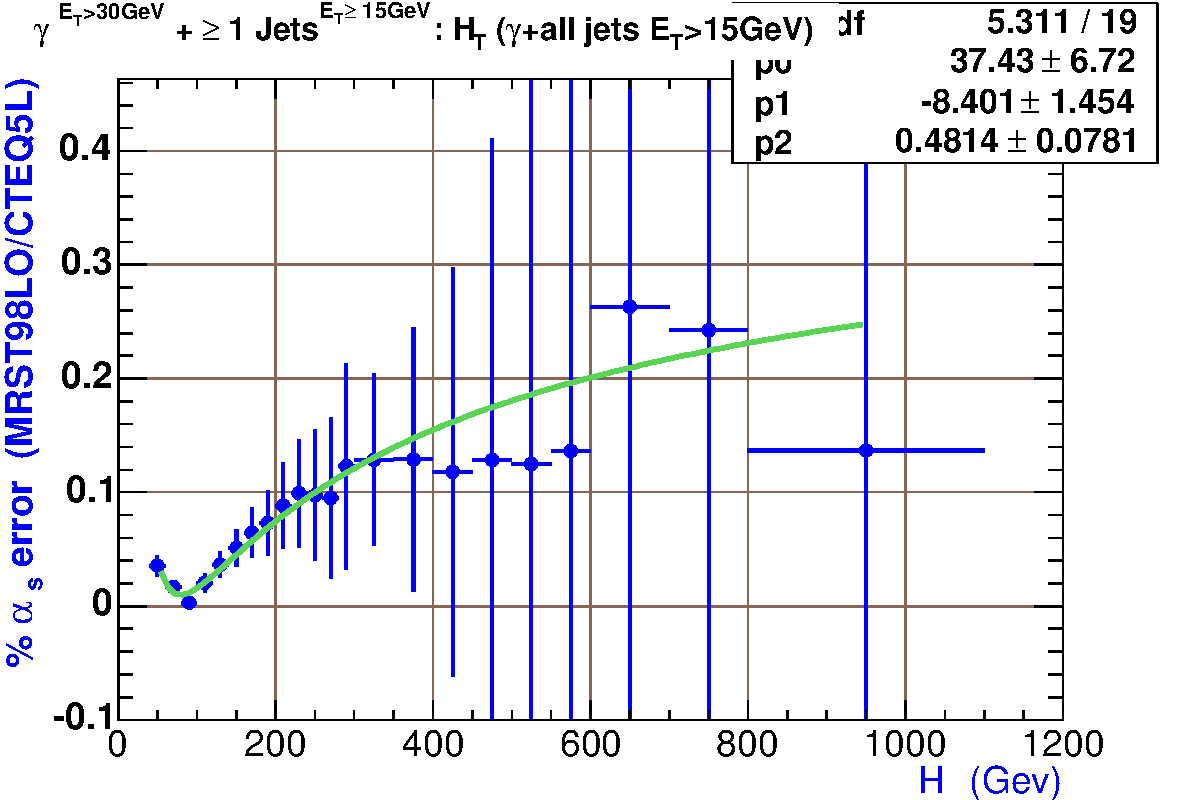
\includegraphics[scale=0.36,keepaspectratio=true]{AlphaSsyst_pj1_Ht.pdf}\hspace{2ex}
 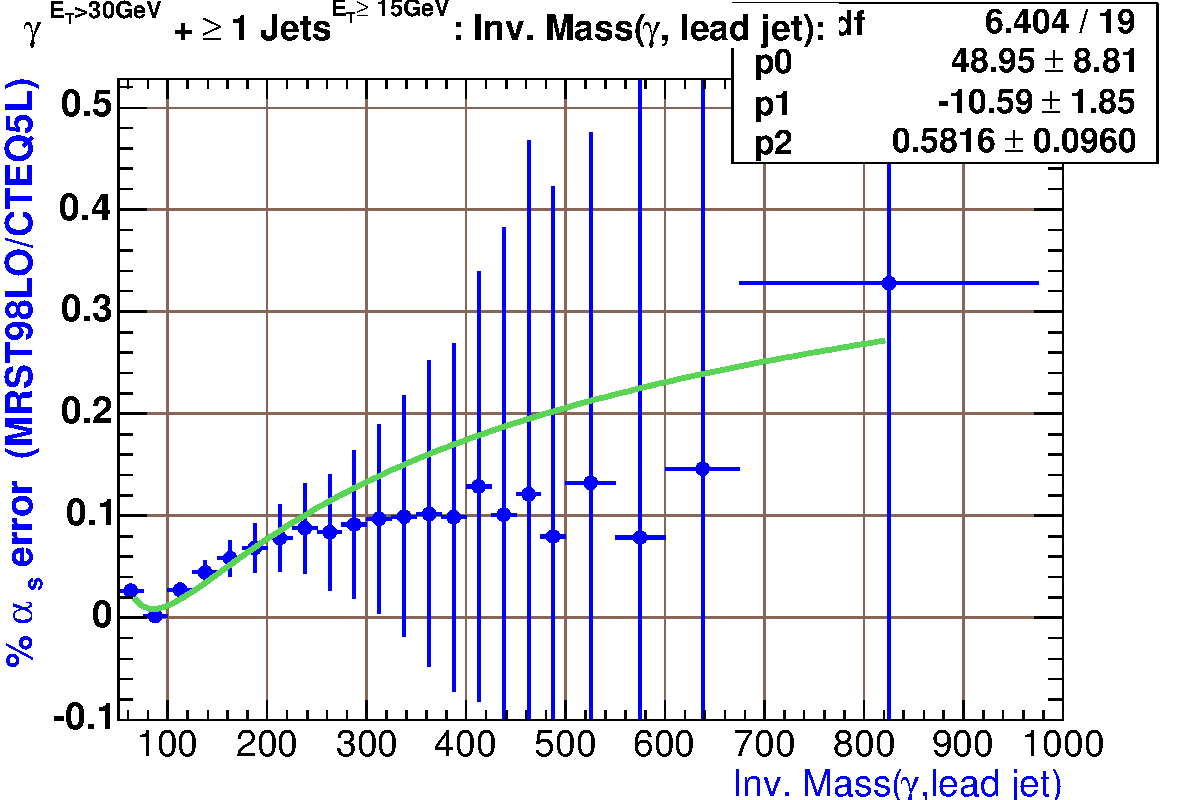
\includegraphics[scale=0.36,keepaspectratio=true]{AlphaS_systpj1_InvM_phojet.pdf}
 \caption{Size of the total \alphas uncertainty for different kinematic distributions in the \phoonejet event sample. The distributions are fitted with a polynomial of the form $p0+p1 \times \sqrt{x})/x+p2$ and used to derive the uncertainty in the final (result) distributions. The function is evaluated at the bin center when deriving the uncertainty for a bin. The total uncertainty ranges from a few percent to about 25\%. The minimum uncertainty is set to be no lower than the first nonzero bin's uncertainty.}
 \label{fig:AlphaS_Syst}
\end{figure}

\section{Luminosity Measurement}
The uncertainty in the measurement of the luminosity is approximately 6\% \cite{www:CLCuncertainty}. This is a combination of the uncertainty in the CLC measurement, beam conditions (orbit and collision points), and measured inelastic cross section.
%[NEED REF. CDF NOTE 6052 (2002) quotes 5\%. there is no update to this note since then.].

Whenever a MC event sample is normalized by the luminosity, the uncertainty in the luminosity measurement needs to be taken into account. This is done by changing the luminosity by $\pm 6\%$ and recalculating the measurement. For every histogram bin, the maximum difference between these altered measurements and the nominal measurement is taken as the uncertainty due to the luminosity. The contribution of this uncertainty to the total uncertainty is relatively small.

\section{Electromagnetic Energy Measurement}
The energy measured by the EM calorimeter carries a 1\% uncertainty. Hence, the photon candidate's energy is shifted by $\pm1\%$ and compared to the nominal distribution. The difference is taken as the systematic uncertainty due to the EM energy measurement.

\section{Cosmic Photon Estimate}
As for the initial test methods, the statistical uncertainty in the cosmic photon template is take as the systematic uncertainty for that bin. This uncertainty is very small and becomes somewhat significant in the high-\met region in the \met measurement.

\section{Beam Halo Photon Estimate}
As this is a very small background, a constant 50\% uncertainty is assigned.

\section{Reweighting Sideband for Method B} \label{sec:sidebandRewgtSyst}
The uncertainty in the reweighting of the sideband events used in Method~B is derived by varying the fake photon fraction by its systematic uncertainty. This will change the fraction of SM $\gamma$ and QCD events chosen. The sideband events are reweighted using these alternate weights and the difference between these and the nominal distribution is taken as the uncertainty. The distribution of alternate weights as a function of photon \et is shown in Fig.~\ref{fig:SidebandPhoEtWgts}.
A second-order parabolic polynomial is used in the fit. This accounts for the uncertainty in the choice of fit function too. This uncertainty increases from a few percent to about 10\% with increasing photon \et.

\begin{figure}[p]
 \centering
 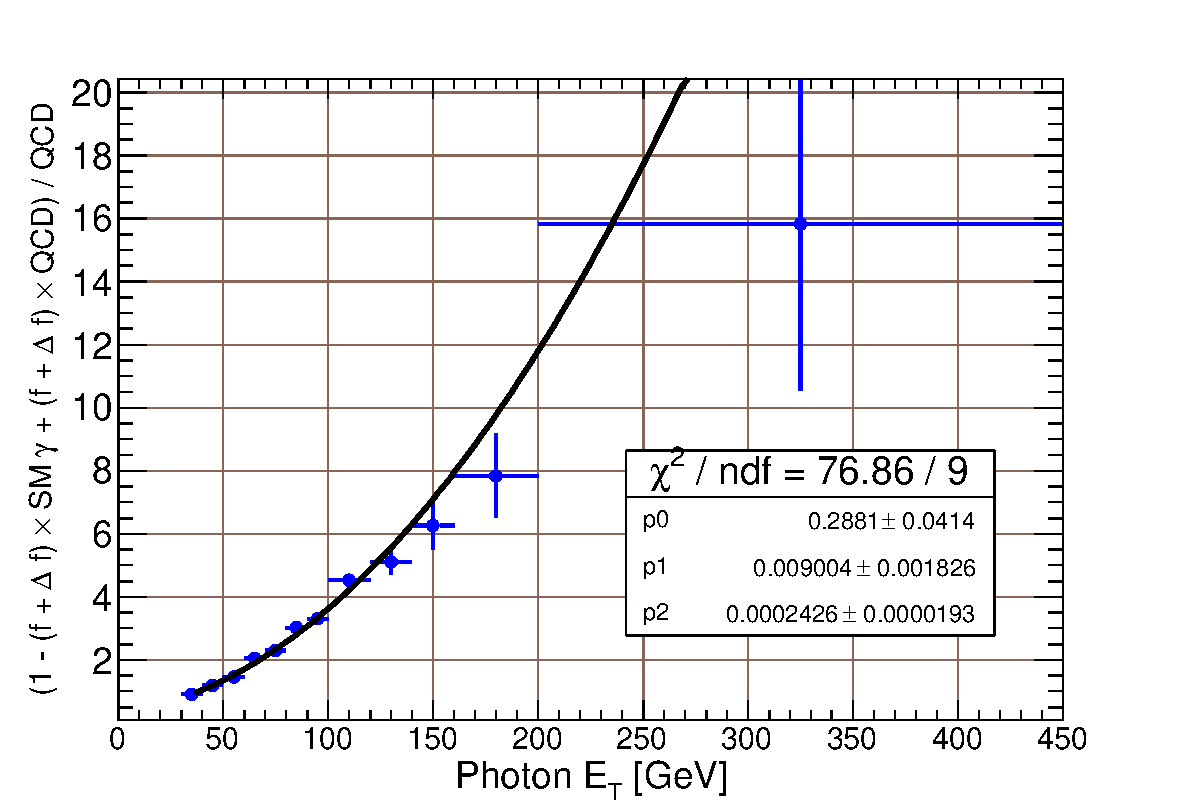
\includegraphics[scale=0.85,keepaspectratio=true]{./MtdB_Sideband_SigmaWeights.pdf}
 \caption{Weights for sideband reweighting in Method B as a function of $E^{\gamma}_{T}$. The SM $\gamma$ and QCD fractions are varied by $f+\Delta f$ as defined by Eq.~\ref{eqa:FakeFraction}. The alternate fit function is of the form $F(E_{T}^{\gamma},f)= p0+p1\times E_{T}^{\gamma}+p2\times(E_{T}^{\gamma})^{2}$.}
 \label{fig:SidebandPhoEtWgts}
\end{figure}

%The fit function is of the form $F(\et^{\gamma},f)= par0+par1\times\et^{\gamma}+par2\times(\et^{\gamma})^{2}$}
%The fit function is of the form $F(\et^{\gamma},\epsilon^{\gamma})= par0+par1\times\sqrt{\et^{\gamma}}+par2\times\et^{\gamma}$ for central weights.
%A second order polynomial $F(\et^{\gamma},\epsilon^{\gamma})= par0+par1\times\et^{\gamma}+par2\times(\et^{\gamma})^{2}$ is used for $+\sigma$ weights. This accounts for the uncertainty in the choice of fit function too.

\section{Total Systematic Uncertainty}
The JES and \alphas uncertainties are the largest systematic uncertainties in most of the measured distributions. Figs.~\ref{fig:g30Jets_Errs_MtdA_plot1_Et_pho}--\ref{fig:g30Jets_Errs_MtdA_plot1_Ht} show the total and fractional systematic uncertainties for the measurements of the \et of the leading photon, \et of the leading jet, invariant mass of the photon and the leading jet, and $H_{T}$, as measured by Method A. The individual systematic uncertainties are color-coded as described by the legend. The top plot shows the absolute total error for the measurement as a function of that measurement. The bottom plot shows the fractional contributions of the individual systematic uncertainties to the total systematic uncertainty. Figs.~\ref{fig:g30Jets_Errs_MtdB_plot1_Et_pho}--\ref{fig:g30Jets_Errs_MtdB_plot1_InvMass_pj1} show the same measurements as measured by Method B, which includes an additional systematic uncertainty due to the reweighting of the sideband events as described in Section~\ref{sec:sidebandRewgtSyst}.

\begin{figure}[p]
 \centering
 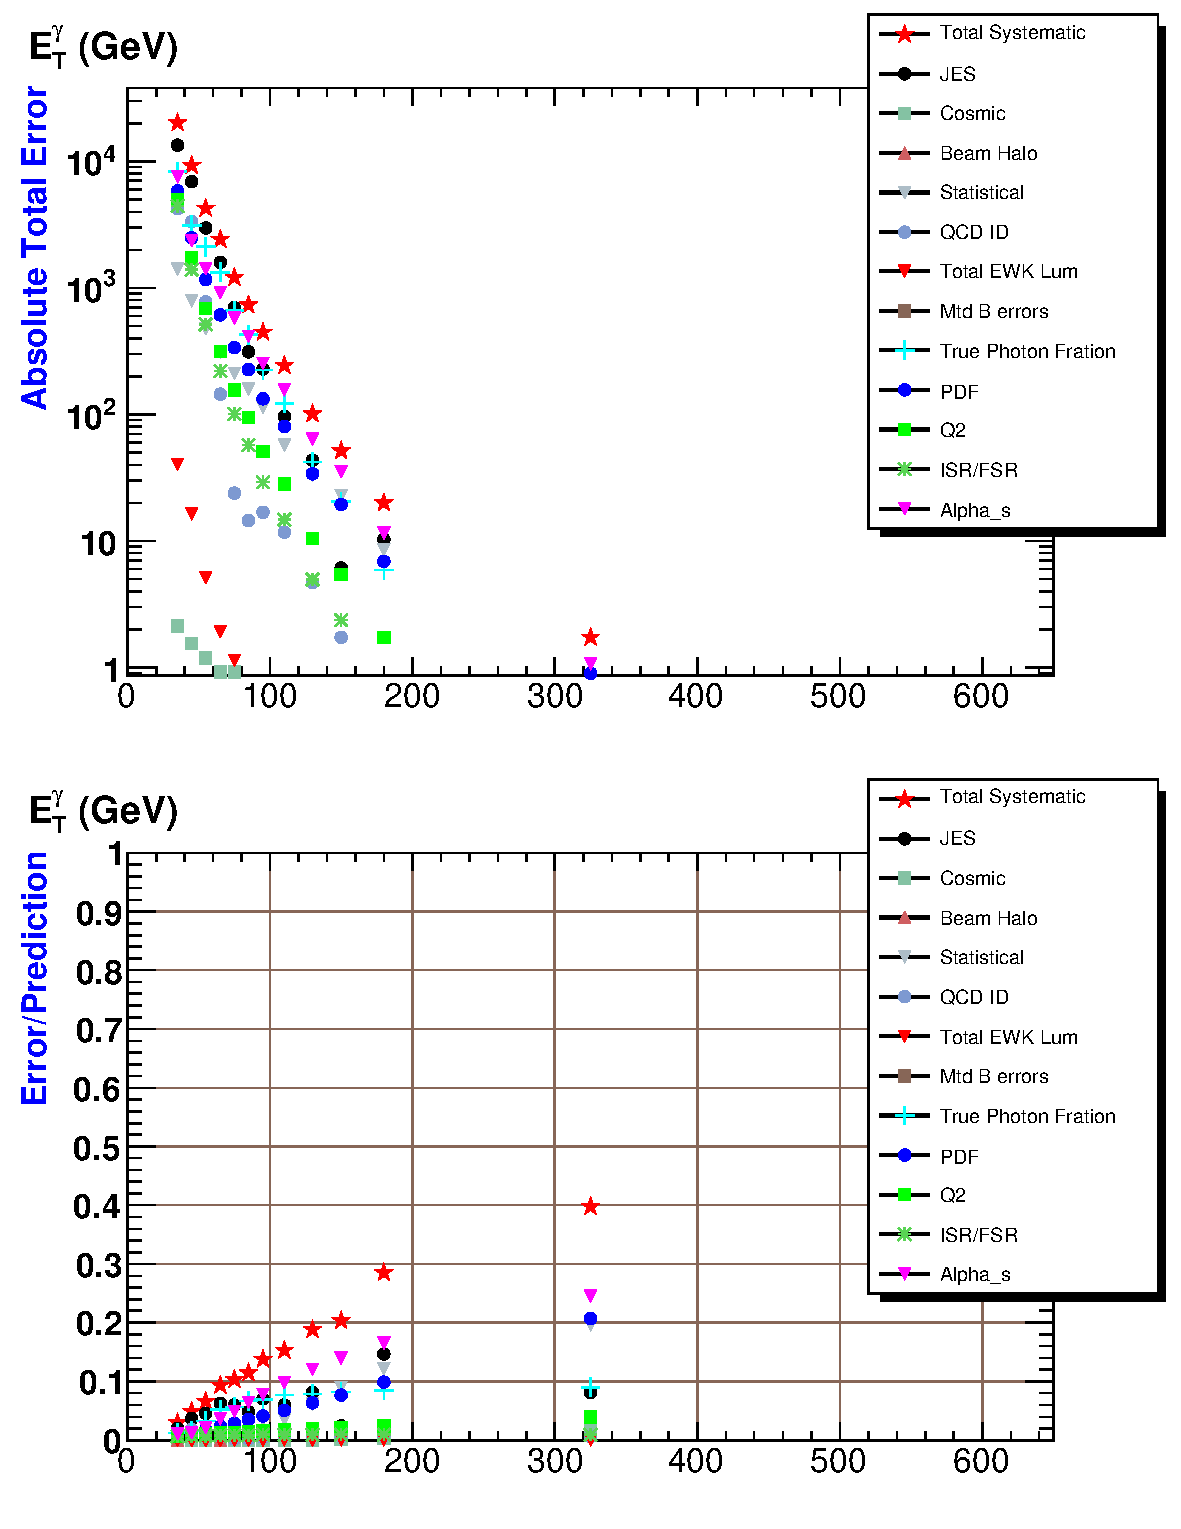
\includegraphics[scale=.7,keepaspectratio=true]{./G30Jets_Errs_MtdA_plot1_Et_pho.pdf}
 % G30Jets_Errs_MtdA_plot1_Et_pho.pdf: 567x734 pixel, 72dpi, 20.00x25.89 cm, bb=0 0 567 734
 \caption{Total and fractional systematic uncertainties for the \et of the leading photon in \phoonejet events as measured by Method A.}
 \label{fig:g30Jets_Errs_MtdA_plot1_Et_pho}
\end{figure}

\begin{figure}[p]
 \centering
 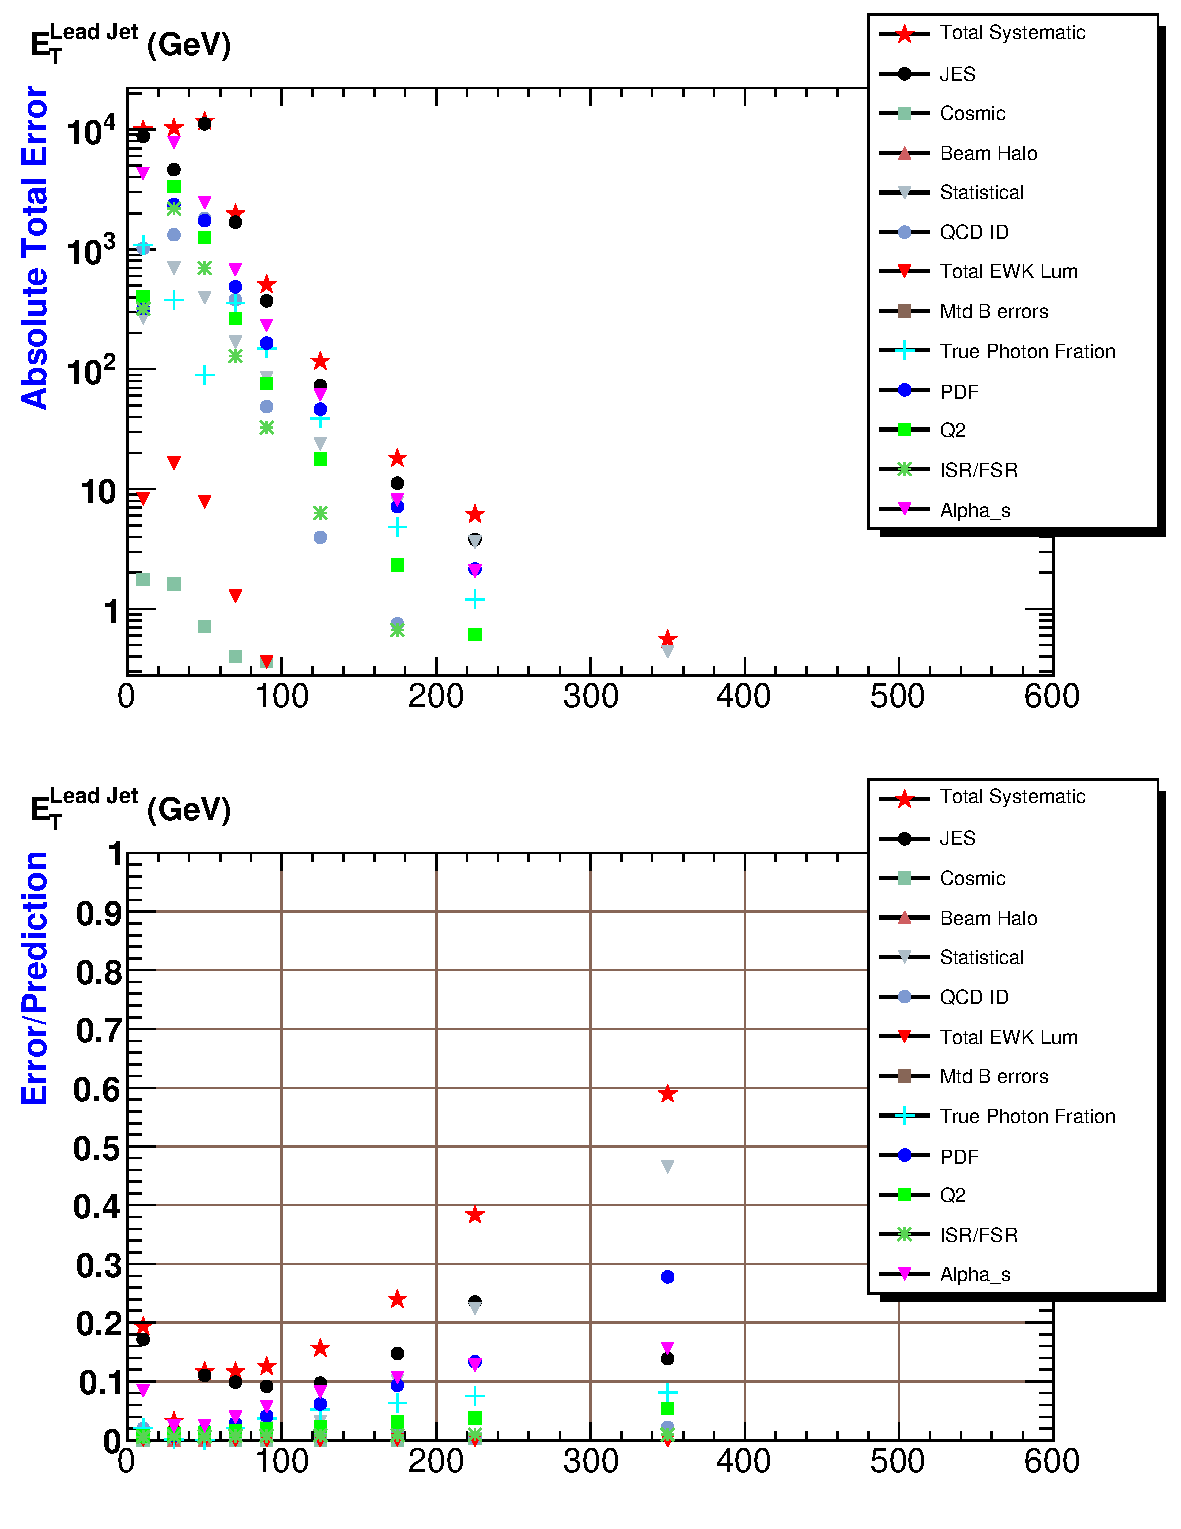
\includegraphics[scale=.7,keepaspectratio=true]{./G30Jets_Errs_MtdA_plot1_Et_j1.pdf}
 % G30Jets_Errs_MtdA_plot1_Et_pho.pdf: 567x734 pixel, 72dpi, 20.00x25.89 cm, bb=0 0 567 734
 \caption{Total and fractional systematic uncertainties for the \et of the leading jet in \phoonejet events as measured by Method A.}
 \label{fig:g30Jets_Errs_MtdA_plot1_Et_jet}
\end{figure}

\begin{figure}[p]
 \centering
 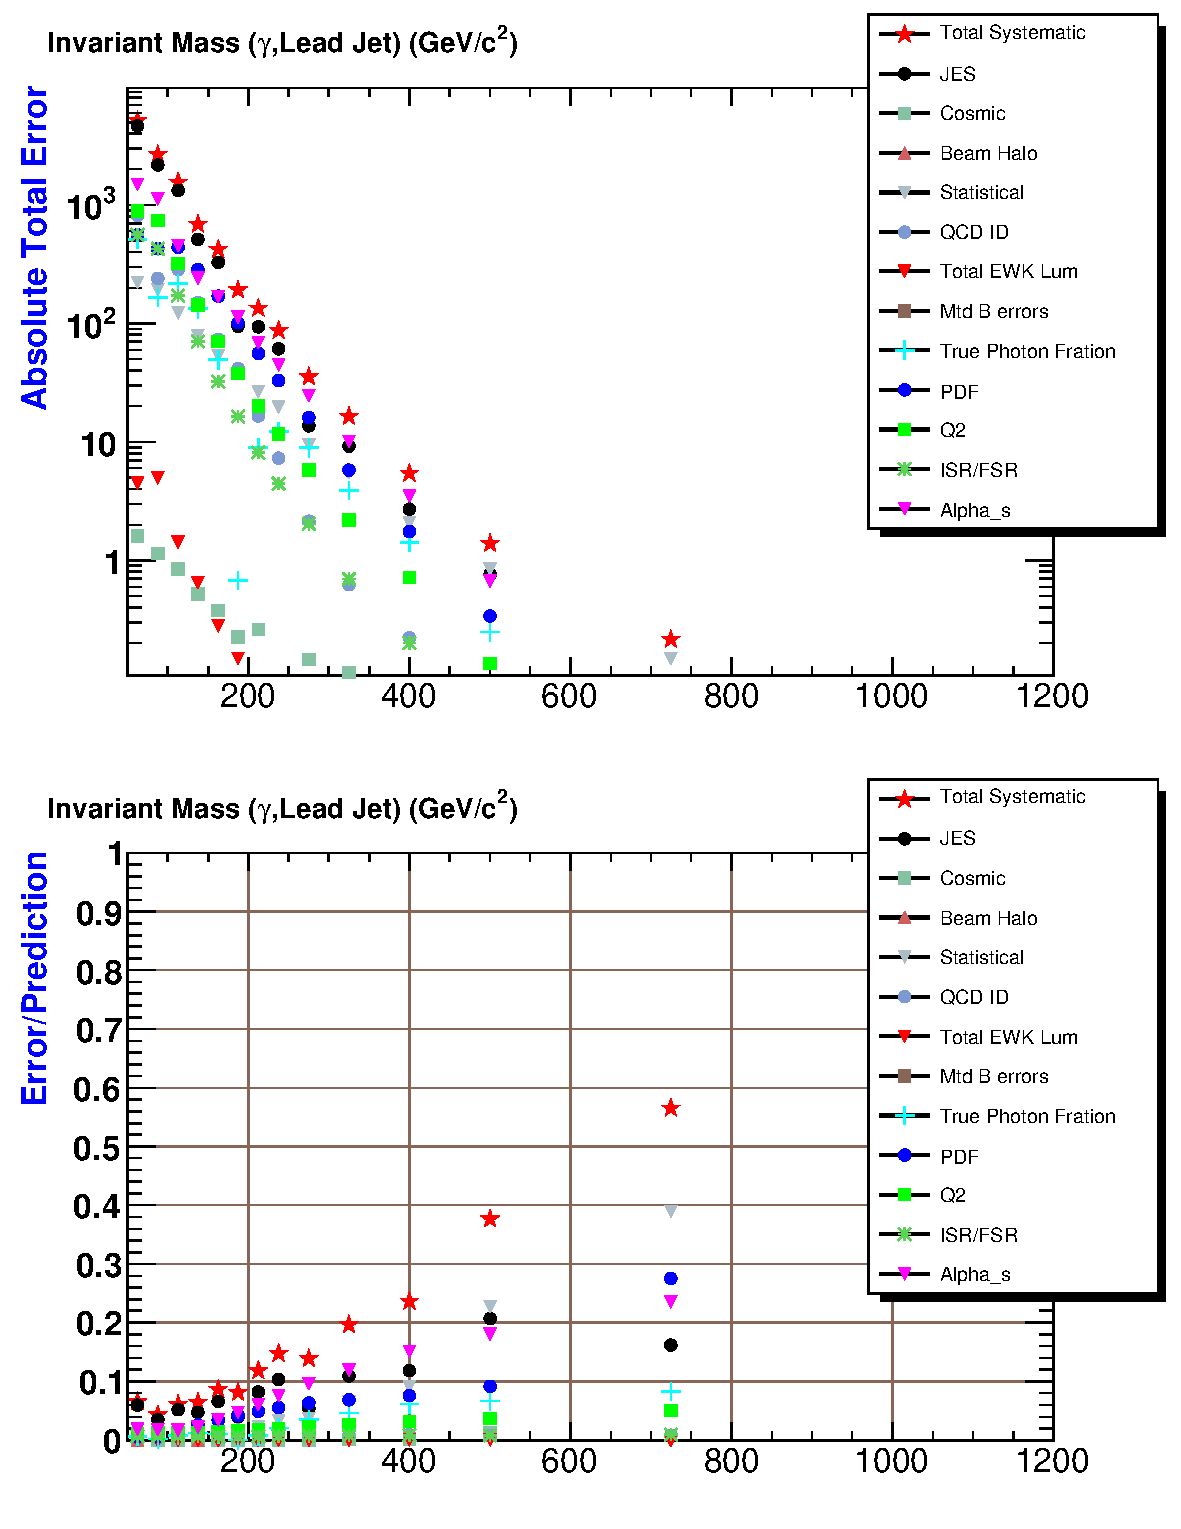
\includegraphics[scale=.7,keepaspectratio=true]{./G30Jets_Errs_MtdA_plot1_InvMass_pj1.pdf}
 % G30Jets_Errs_MtdA_plot1_Et_pho.pdf: 567x734 pixel, 72dpi, 20.00x25.89 cm, bb=0 0 567 734
 \caption{Total and fractional systematic uncertainties for the invariant mass of the photon and the leading jet in \phoonejet events as measured by Method A.}
 \label{fig:g30Jets_Errs_MtdA_plot1_InvMass_pj1}
\end{figure}

\begin{figure}[p]
 \centering
 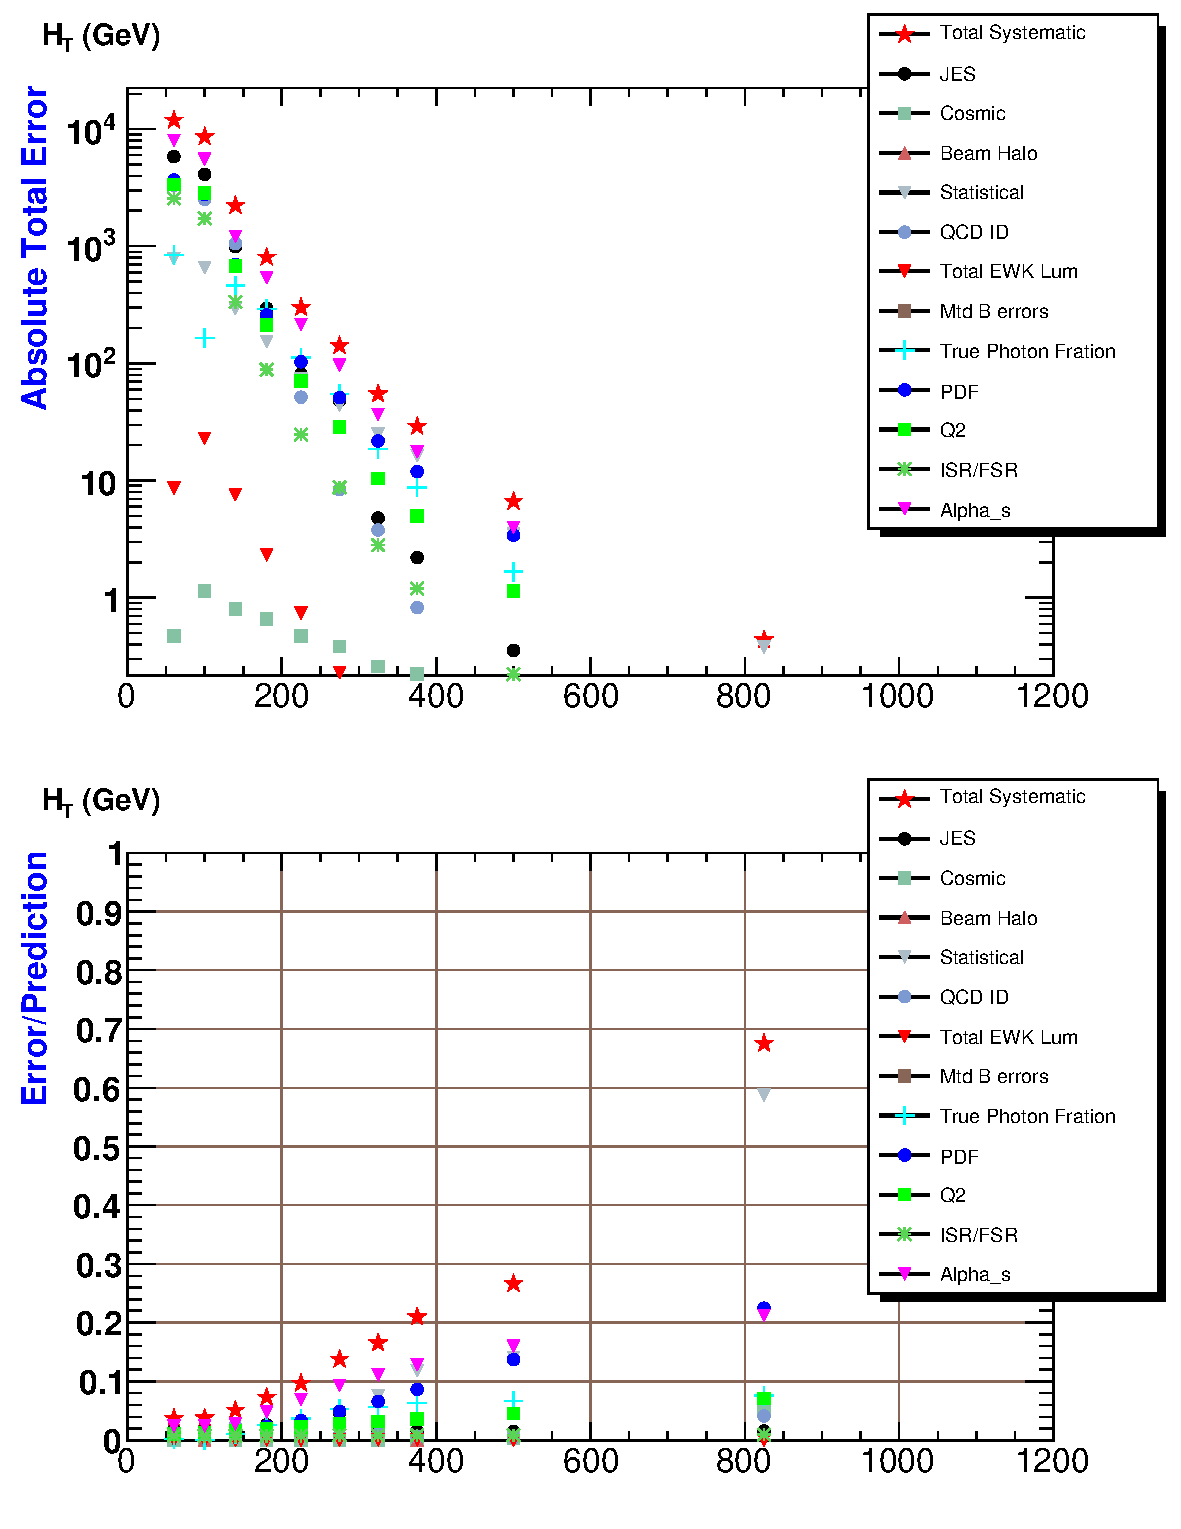
\includegraphics[scale=.7,keepaspectratio=true]{./G30Jets_Errs_MtdA_plot1_Ht.pdf}
 % G30Jets_Errs_MtdA_plot1_Et_pho.pdf: 567x734 pixel, 72dpi, 20.00x25.89 cm, bb=0 0 567 734
 \caption{Total and fractional systematic uncertainties for the $H_{T}$ measurement in \phoonejet events as measured by Method A.}
 \label{fig:g30Jets_Errs_MtdA_plot1_Ht}
\end{figure}

\begin{figure}[p]
 \centering
 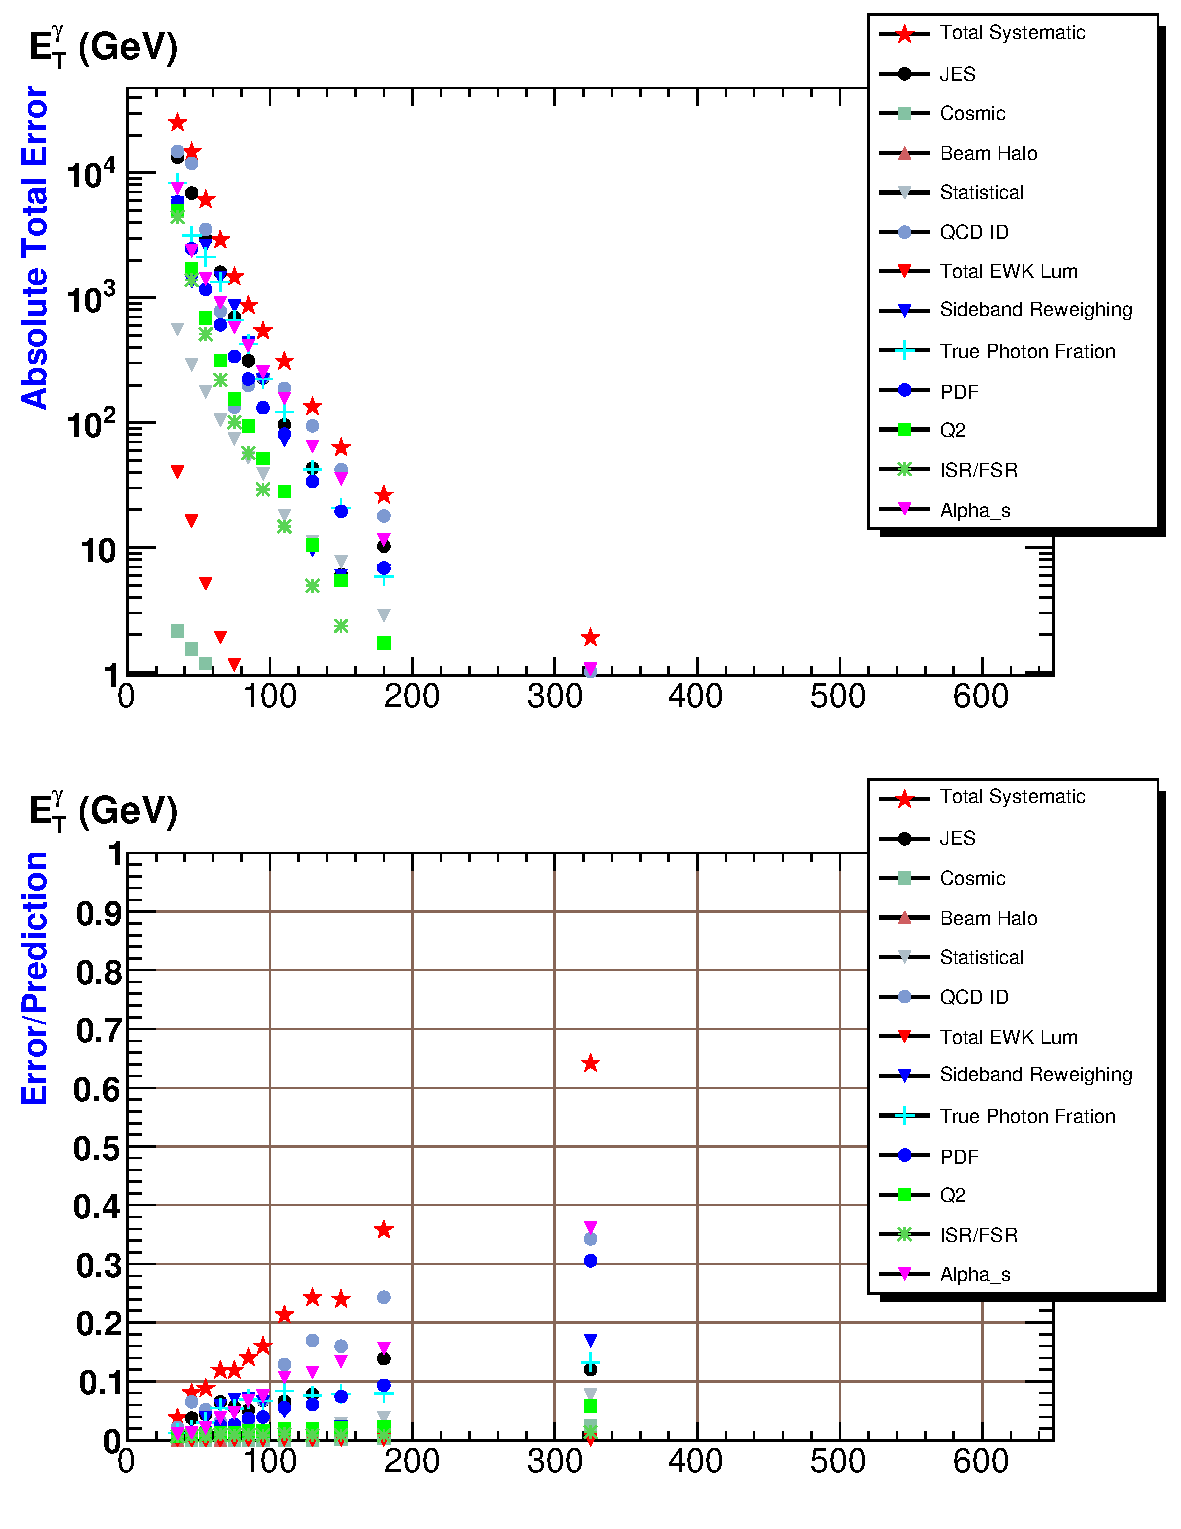
\includegraphics[scale=.7,keepaspectratio=true]{./G30Jets_Errs_MtdB_plot1_Et_pho.pdf}
 % G30Jets_Errs_MtdA_plot1_Et_pho.pdf: 567x734 pixel, 72dpi, 20.00x25.89 cm, bb=0 0 567 734
 \caption{Total and fractional systematic uncertainties for the \et of the leading photon in \phoonejet events as measured by Method B.}
 \label{fig:g30Jets_Errs_MtdB_plot1_Et_pho}
\end{figure}

\begin{figure}[p]
 \centering
 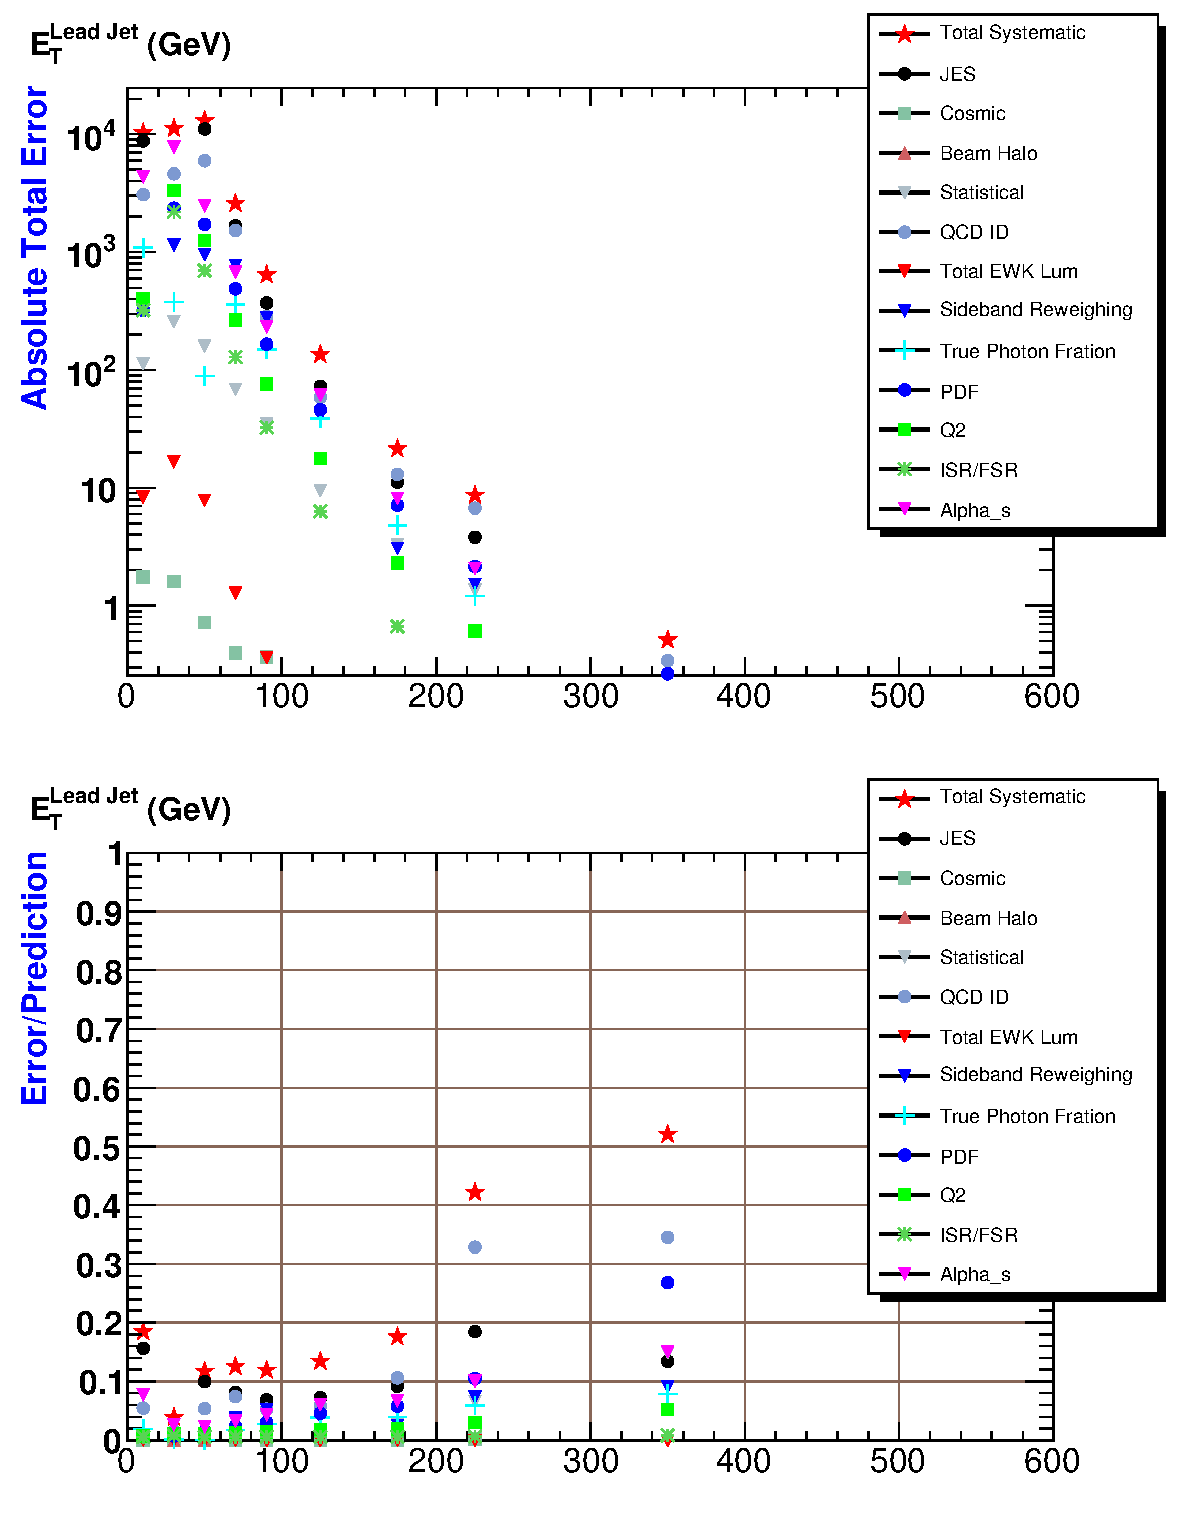
\includegraphics[scale=.7,keepaspectratio=true]{./G30Jets_Errs_MtdB_plot1_Et_j1.pdf}
 % G30Jets_Errs_MtdA_plot1_Et_pho.pdf: 567x734 pixel, 72dpi, 20.00x25.89 cm, bb=0 0 567 734
 \caption{Total and fractional systematic uncertainties for the \et of the leading jet in \phoonejet events as measured by Method B.}
 \label{fig:g30Jets_Errs_MtdB_plot1_Et_jet}
\end{figure}

\begin{figure}[p]
 \centering
 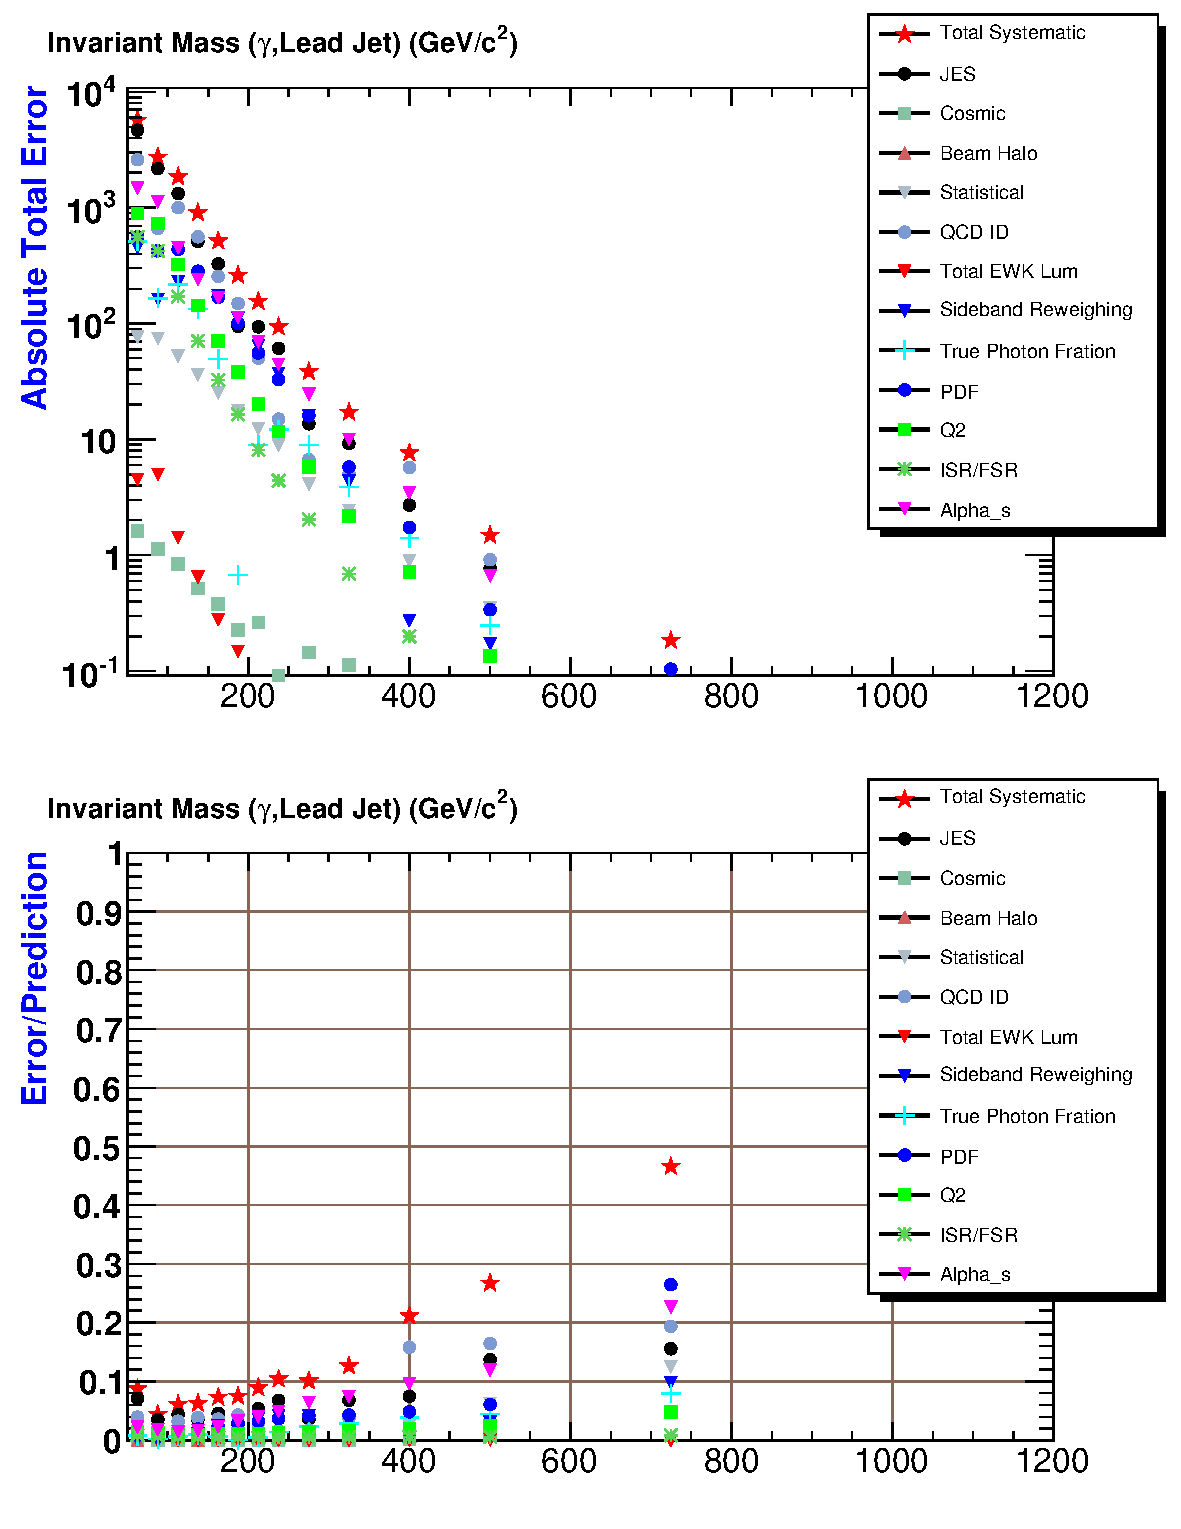
\includegraphics[scale=.7,keepaspectratio=true]{./G30Jets_Errs_MtdB_plot1_InvMass_pj1.pdf}
 % G30Jets_Errs_MtdA_plot1_Et_pho.pdf: 567x734 pixel, 72dpi, 20.00x25.89 cm, bb=0 0 567 734
 \caption{Total and fractional systematic uncertainties for the invariant mass of the photon and the leading jet in \phoonejet events as measured by Method B.}
 \label{fig:g30Jets_Errs_MtdB_plot1_InvMass_pj1}
\end{figure}



